\documentclass[11pt]{article}

% Paquetes
%===================================================================================================

% Paquete para incluir codigo
\usepackage{listings}

% Paquete para incluir imagenes
\usepackage{graphicx}
\graphicspath{ {./Imagenes/} }

% Para fijar las imagenes en la posicion deseada
\usepackage{float}

% Para que el codigo acepte caracteres en utf8
\lstset{literate=
  {á}{{\'a}}1 {é}{{\'e}}1 {í}{{\'i}}1 {ó}{{\'o}}1 {ú}{{\'u}}1
  {Á}{{\'A}}1 {É}{{\'E}}1 {Í}{{\'I}}1 {Ó}{{\'O}}1 {Ú}{{\'U}}1
  {à}{{\`a}}1 {è}{{\`e}}1 {ì}{{\`i}}1 {ò}{{\`o}}1 {ù}{{\`u}}1
  {À}{{\`A}}1 {È}{{\'E}}1 {Ì}{{\`I}}1 {Ò}{{\`O}}1 {Ù}{{\`U}}1
  {ä}{{\"a}}1 {ë}{{\"e}}1 {ï}{{\"i}}1 {ö}{{\"o}}1 {ü}{{\"u}}1
  {Ä}{{\"A}}1 {Ë}{{\"E}}1 {Ï}{{\"I}}1 {Ö}{{\"O}}1 {Ü}{{\"U}}1
  {â}{{\^a}}1 {ê}{{\^e}}1 {î}{{\^i}}1 {ô}{{\^o}}1 {û}{{\^u}}1
  {Â}{{\^A}}1 {Ê}{{\^E}}1 {Î}{{\^I}}1 {Ô}{{\^O}}1 {Û}{{\^U}}1
  {ã}{{\~a}}1 {ẽ}{{\~e}}1 {ĩ}{{\~i}}1 {õ}{{\~o}}1 {ũ}{{\~u}}1
  {Ã}{{\~A}}1 {Ẽ}{{\~E}}1 {Ĩ}{{\~I}}1 {Õ}{{\~O}}1 {Ũ}{{\~U}}1
  {œ}{{\oe}}1 {Œ}{{\OE}}1 {æ}{{\ae}}1 {Æ}{{\AE}}1 {ß}{{\ss}}1
  {ű}{{\H{u}}}1 {Ű}{{\H{U}}}1 {ő}{{\H{o}}}1 {Ő}{{\H{O}}}1
  {ç}{{\c c}}1 {Ç}{{\c C}}1 {ø}{{\o}}1 {å}{{\r a}}1 {Å}{{\r A}}1
  {€}{{\euro}}1 {£}{{\pounds}}1 {«}{{\guillemotleft}}1
  {»}{{\guillemotright}}1 {ñ}{{\~n}}1 {Ñ}{{\~N}}1 {¿}{{?`}}1 {¡}{{!`}}1
}

% Para que los metadatos que escribe latex esten en español
\usepackage[spanish]{babel}

% Para la bibliografia
% Sin esto, los enlaces de la bibliografia dan un error de compilacion
\usepackage{url}

% Para mostrar graficas de dos imagenes, cada una con su caption, y con un caption comun
\usepackage{subcaption}

% Metadatos del documento
%===================================================================================================
\title{
    {Aprendizaje Automático - Segunda Práctica}\\
    {Complejidad de $H$ y el ruido}\\
    {Modelos Lineales}
}

\author{
    {Sergio Quijano Rey - 72103503k}\\
    {4º Doble Grado Ingeniería Informática y Matemáticas}\\
    {sergioquijano@correo.ugr.es}
}

\date{\today}

% Separacion entre parrafos
\setlength{\parskip}{1em}


% Contenido del documento
%===================================================================================================
\begin{document}

% Portada del documento
\maketitle
\pagebreak

% Indice de contenidos
\tableofcontents
\pagebreak

\section{Ejercicio 1 - Sobre la complejidad de $H$ el ruido}

\subsection{Observaciones iniciales}

Para este primer ejercicio, hacemos uso de tres funciones que se nos dan en el fichero \lstinline{template_trabajo2.py}. Las dos primeras funciones devuelven una lista de $N$ vectores de una dimensión dada.

\begin{itemize}
    \item \lstinline{simula_unif}: genera una lista de $N$ vectores aleatorios de una dimensión dada. La distribución aleatoria que siguen es una distribución uniforme en un intervalo dado
    \item \lstinline{simula_gauss}: genera una lista de $N$ vectores aleatorios de dimensión dada. La distribución aleatoria es una normal de media cero y varianza dada
    \item \lstinline{simula_recta}: genera una recta aleatoria que pasa a través de un intervalo 2-dimensional dado
\end{itemize}

Además, al principio de cada función asociada a los ejercicios (\lstinline{ejercicio1()}, \lstinline{ejercicio2()}, \lstinline{ejercicio_bonus()}) establecemos una semilla aleatoria fija con la orden \lstinline{np.random.seed(123456789)}. Así, los resultados que obtenemos serán reproducibles. Aunque por estar usando probablemente distintos configuraciones de sistemas operativos, hardware, versión de \lstinline{python}, \ldots, los resultados obtenidos por los profesores de prácticas no serán exactamente los mismos cuando exista un factor aleatorio.

\subsection{Apartado 1}

En este apartado se pide que dibujemos las nubes de puntos simuladas con las dos primeras funciones dadas por los profesores. Para ello empleamos los siguientes parámetros:

\begin{itemize}
    \item $N = 50$
    \item $dim = 2$
    \item $rango = [-50, 50]$
    \item $\sigma = [5, 7]$ donde $\sigma$ indica la varianza (por tanto sería más adecuada la notación $\sigma^2$) en el eje $x$ e $y$
\end{itemize}

Lanzando el código obtenemos las dos siguientes nubes de puntos:

\begin{figure}[h]
    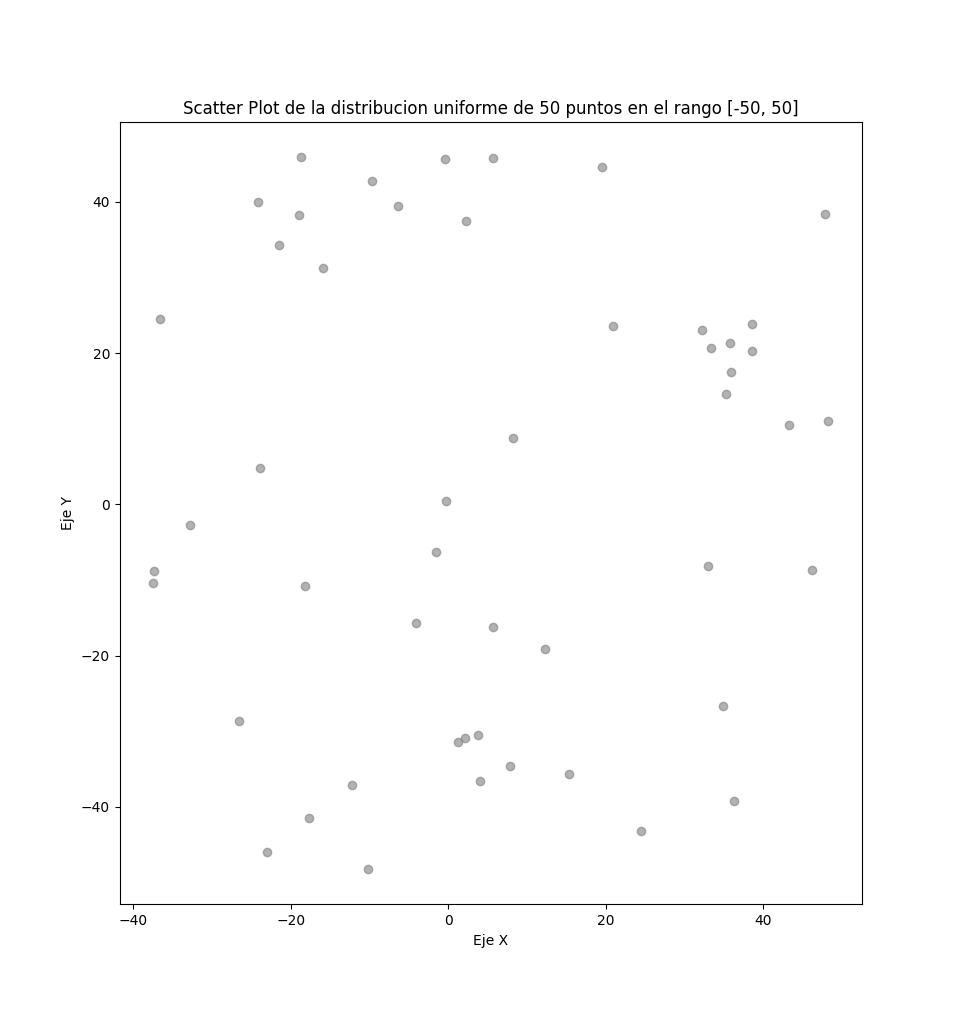
\includegraphics[width=0.60 \textwidth]{nube_puntos_uniforme}
    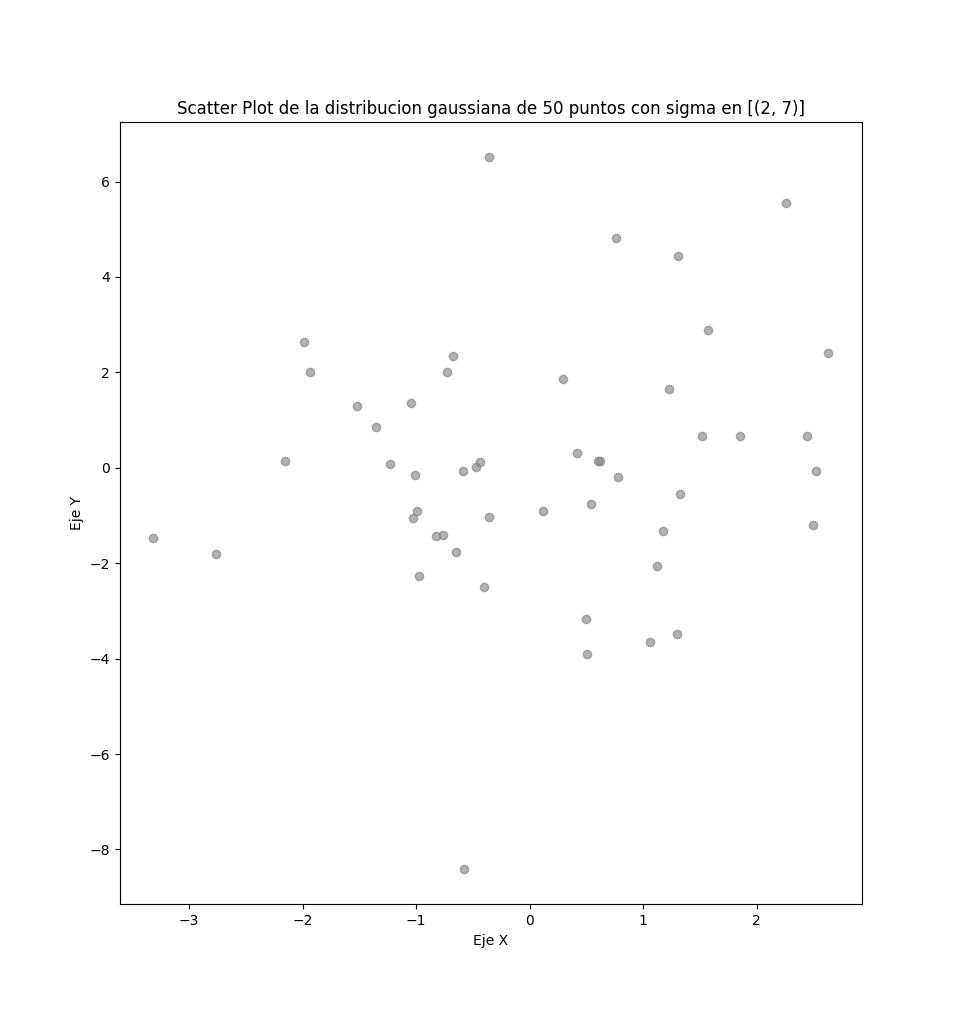
\includegraphics[width=0.60 \textwidth]{nube_puntos_normal}
    \caption{Nubes de puntos de las dos distribuciones}
\end{figure}

\subsection{Apartado 2}

Vamos a valorar la influencia del ruido en la selección dela complejidad de la clase de funciones. Para ello generamos una muestra de puntos bidimensionales. En concreto, generamos 100 puntos en el intervalo $[-50, 50]$.

Una vez que generamos esta muestra de datos, los etiquetamos usando una recta generada aleatoriamente, usando la función dada por los profesores \lstinline{simula_recta}. Con la recta $f(x) = ax + b$, etiquetamos los datos con la función de etiquetado $(x, y) \rightarrow sign(y - ax - b)$. Esta función toma un punto $x, y$, calcula su distancia a la recta $f$ (que se corresponde con $y - f(x)$) y como etiqueta asigna el signo de esta distancia. Es decir, estamos mirando si un punto se queda por encima de la recta (etiqueta $+1$) o por debajo (etiqueta $-1$).

\textbf{Observación importante}: en el subapartado c), hemos considerado una interpretación alternativa del ejercicio, pues parece tener más interés académico a la hora de analizar las propiedades de las funciones que se nos dan para clasificar. Por tanto, desarrollamos una sección \ref{section:apartado_obligatorio}, donde realizamos la tarea especificada, y una sección \ref{section:apartado_extra} donde realizamos el experimento alternativo. Ambos procesos nos parecen pobres a la hora de extraer información sobre dichas funciones (como se comentará en el análisis de cada uno de los subapartados), pero la interpretación alternativa parece dar algo más de juego para realizar los análisis.

\subsubsection{Subapartado a)} \label{section:ejercicio1.2.a}

El enunciado de este apartado especifica que se vuelva a generar la muestra de datos, como se especifica anteriormente, o al menos así lo hemos interpretado. Por tanto, se puede ver que la nube de datos no es la misma que la nube de datos uniforme del Apartado 1.

La gráfica de los datos etiquetados, junto a la recta que se usa para etiquetar, es la siguiente:

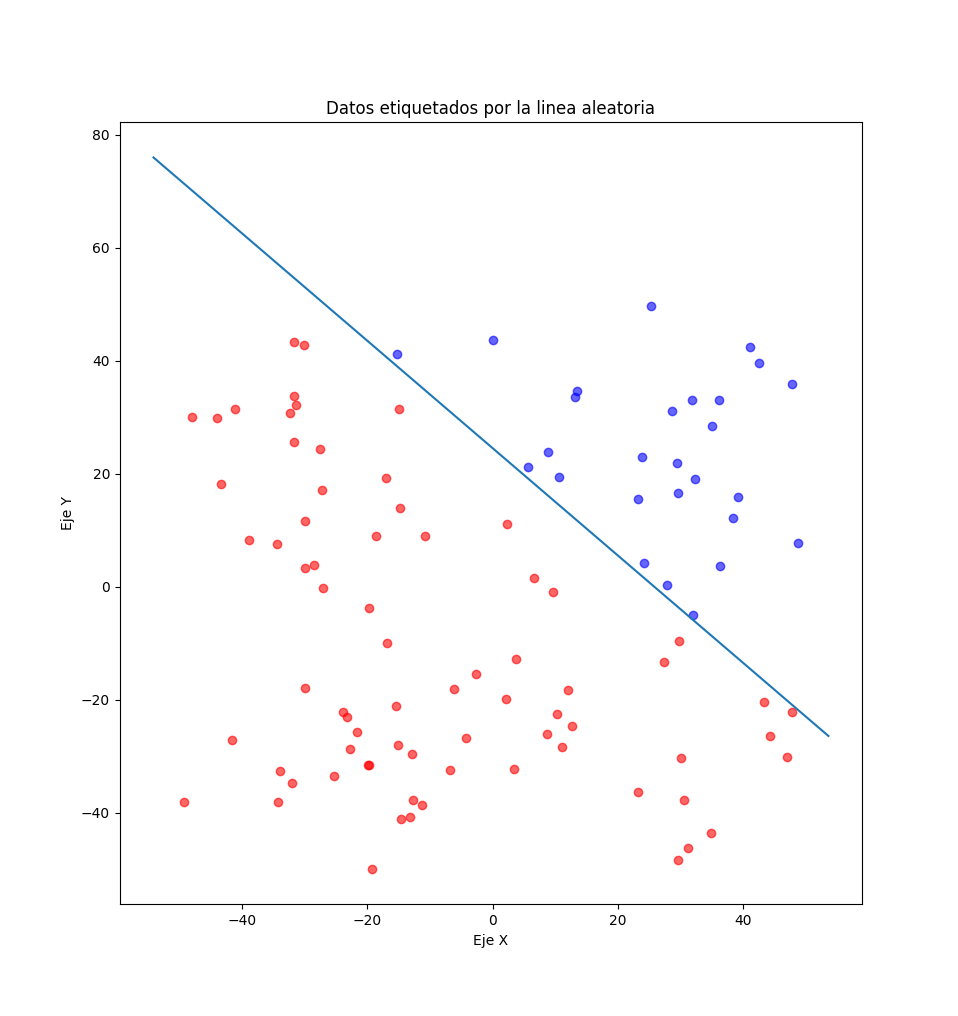
\includegraphics[width=0.9 \textwidth]{puntos_clasificados_recta01}

La gráfica deja claro que los puntos han sido correctamente clasificados a partir de la recta generada aleatoriamente.

\subsubsection{Subapartado b)} \label{section:ejercicio1.2.b}

Modificamos el 10\% de las etiquetas positivas y un 10\% de las etiquetas negativas, y volvemos a mostrar la gráfica.

Para realizar esto de forma eficiente, lo que hacemos es tomar dos vectores, uno con las posiciones de etiquetas positivas y otro con las posiciones de las etiquetas negativas. Calculamos el número de etiquetas de cada tipo a cambiar ($N_1, N_2$), a partir de un porcentaje arbitrario (para nuestro caso concreto, usamos $0.1$). Hacemos un \emph{shuffle} de los dos vectores de posiciones y cambiamos el etiquetado de las $N_1$ y $N_2$ primeras posiciones del vector remezclado. Con ello modificamos un porcentaje dado de las etiquetas de forma aleatoria. Todo esto se puede ver en la función \lstinline{change_labels}.

Notar que podemos tener clases sin puntos. Es decir, que no etiquetamos ningún dato con o bien $+1$ o bien $-1$. En el caso de la recta, es muy improbable que esto pase. Pero en el siguiente subapartado, con ciertas funciones es muy probable que pase.

El gráfico de clasificación tras esta modificación aleatoria es:

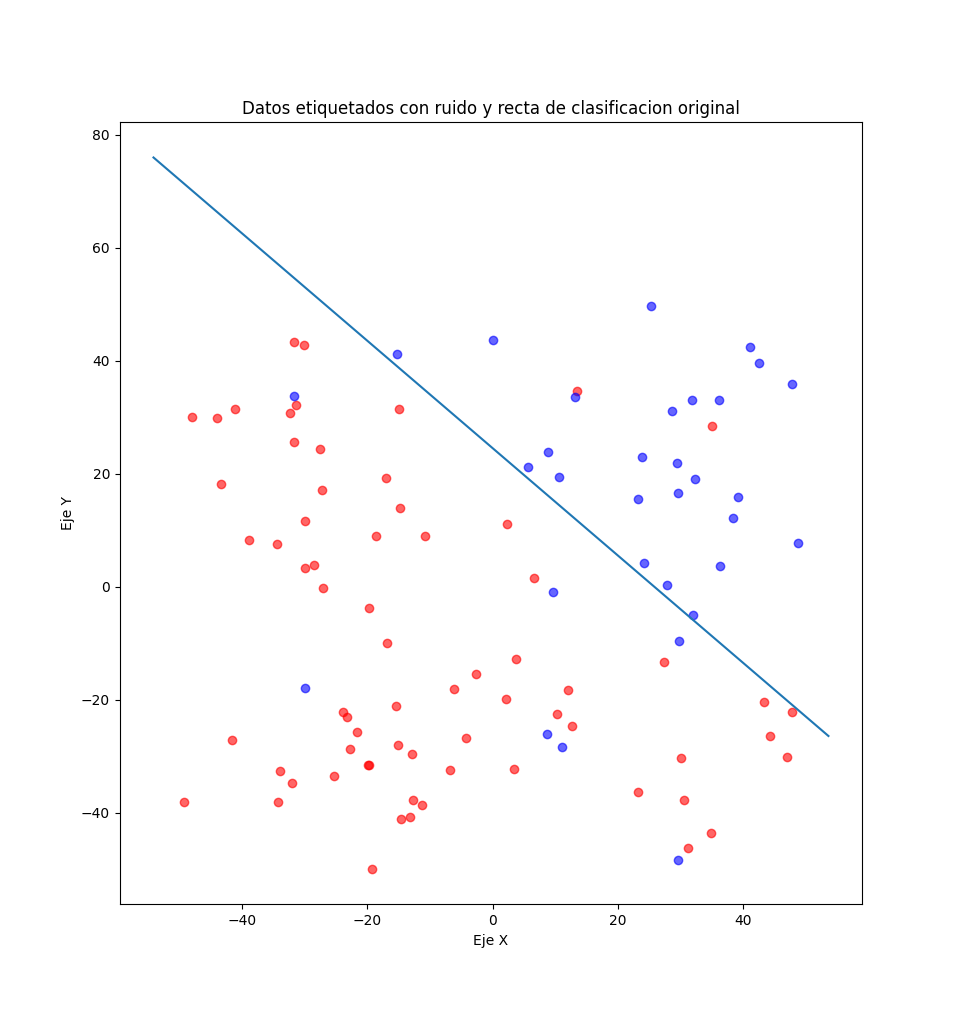
\includegraphics[width = 0.8 \textwidth]{puntos_clasificados_recta_aleatorizados01}

Se ve con claridad cómo esta operación introduce ruido sobre nuestras etiquetas. Aproximadamente, tendremos un error entorno al 10\% por la forma en la que hemos modificado las etiquetas (dependendiendo del ratio positivos / negativos, el error porcentual puede ser de hasta el 9\%).

\subsubsection{Subapartado c)} \label{section:apartado_obligatorio}

En este apartado, debemos considerar las siguientes funciones que definen una frontera de clasificación:

\begin{itemize}
    \item $f_0(x, y):= (x - 10)^2 + (y - 20)^2 - 400$
    \item $f_1(x, y):= \frac{1}{2} (x + 10)^2 + (y - 20)^2 - 400$
    \\item $f_2(x, y):= \frac{1}{2} (x - 10)^2 - (y + 20)^2 - 400$
    \item $f_3(x, y):= y - 20x^2 -5x +3$
\end{itemize}

Estas funciones no van a modificar el etiquetado que ya teníamos (el generado a partir de una recta y la introducción sintética de ruido). Simplemente mostramos las regiones de clasificación de estas nuevas funciones y los puntos con el clasificado original, buscando asi realizar un análisis sobre el uso de estos clasificadores más complejos.

Podríamos haber intentado mostras las líneas de frontera de etiquetado, como hemos hecho con la recta. Pero para ello, tenemos que calcular un despeje de $f(x, y)$, o bien de $x$ o bien de $y$, pues $f(x, y)$ viene dada de forma implícita. No todas las funciones tienen un despeje global, por lo que habría que emplear el teorema de la función implícita para realizar despejes locales, y después concatenar las graficas obtenidas con los despejes locales. Hemos considerado que esto entorpecía demasiado el código. Así que la solución encontrada ha sido usar la función \lstinline{contourf} de la librería \lstinline{matplotlib.pyplot}, con la que pintaremos las regiones en las que clasificamos positivamente y las regiones en las que clasificamos negativamente.

Una vez hechos estos comentarios, mostramos las gráficas obtenidas como se nos pedía:

\begin{figure}[H]
    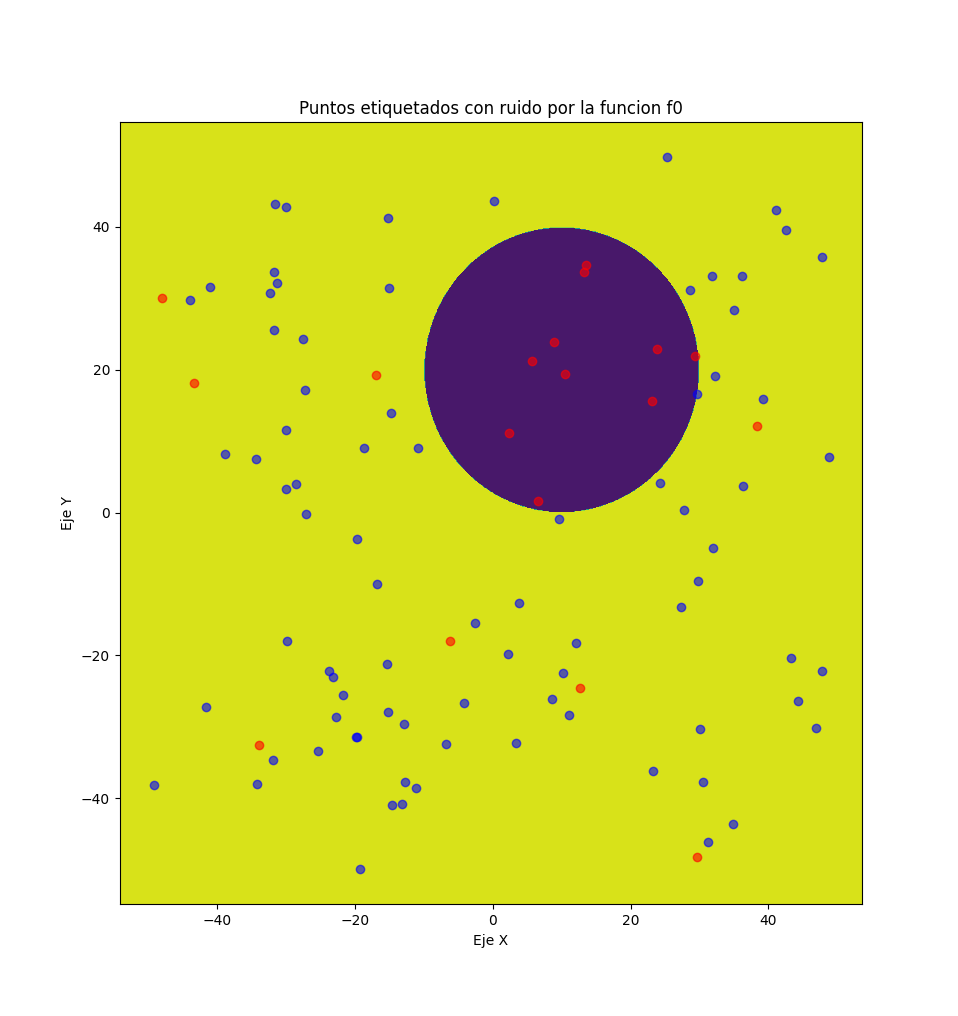
\includegraphics[width=0.60 \textwidth]{puntos_clasificados_f0.png}
    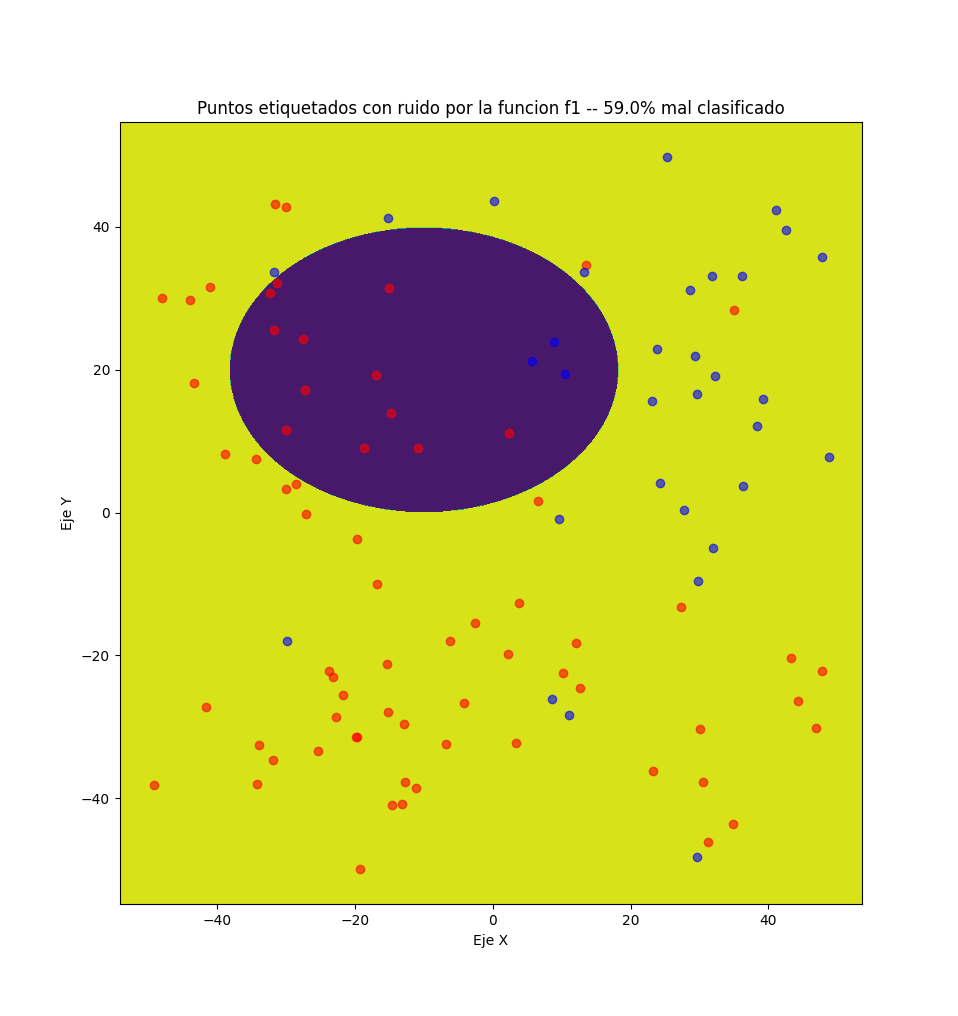
\includegraphics[width=0.60 \textwidth]{puntos_clasificados_f1.png}

    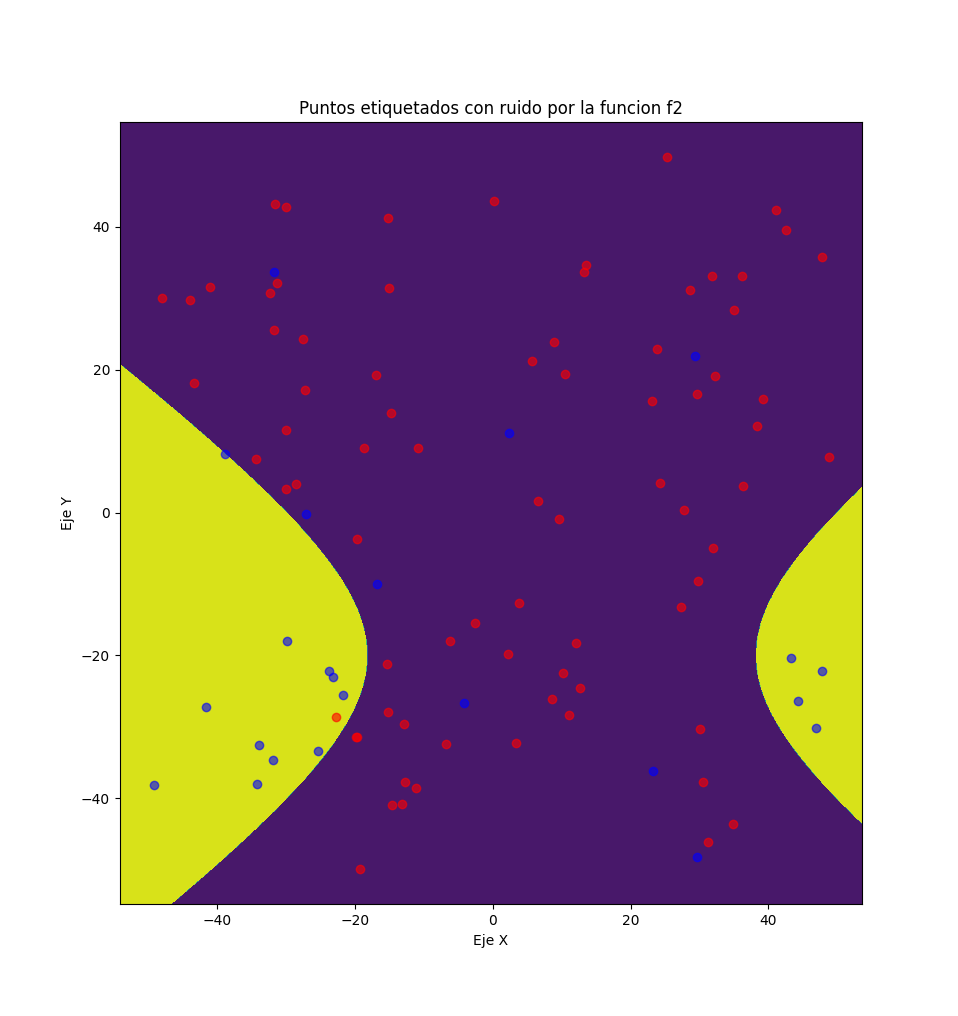
\includegraphics[width=0.60 \textwidth]{puntos_clasificados_f2.png}
    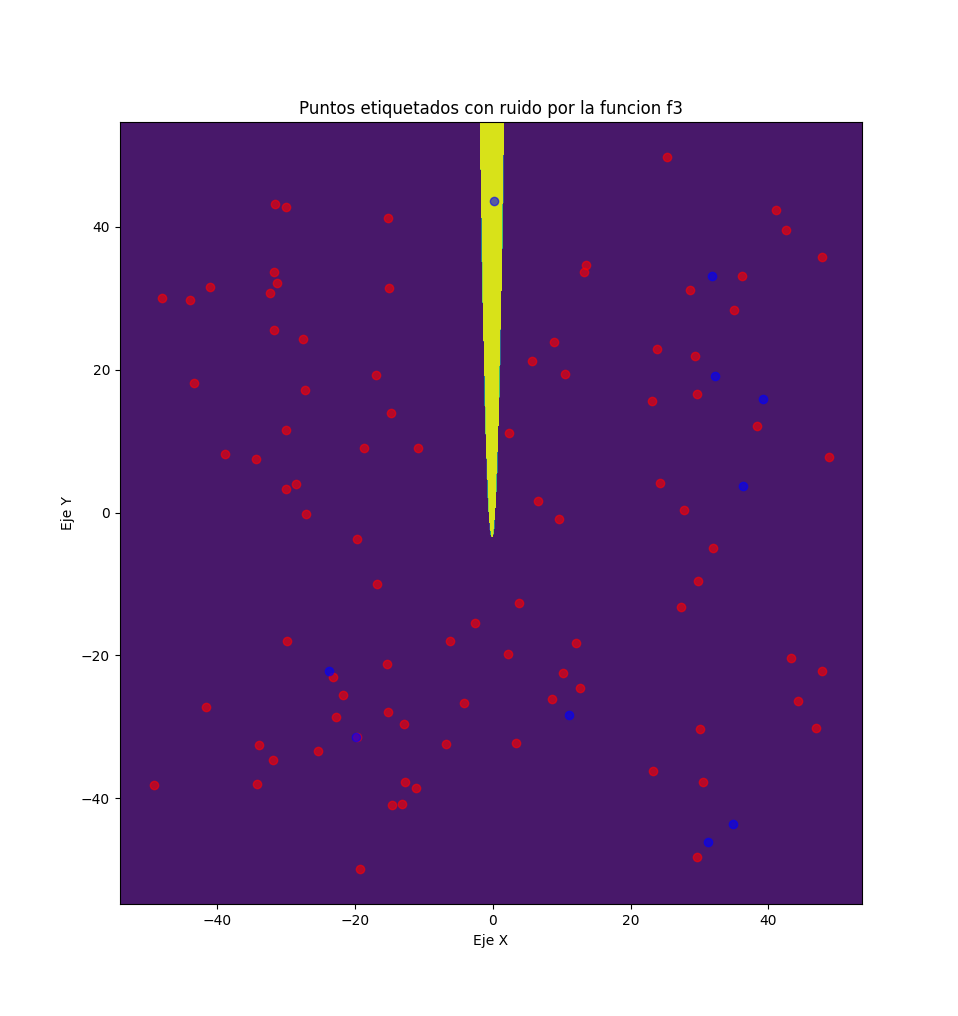
\includegraphics[width=0.60 \textwidth]{puntos_clasificados_f3.png}

    \caption{Etiquetado original sobre las nuevas funciones de etiquetado}
\end{figure}

% TODO -- Mirar la discusión que hago en el experimento, porque unas cuantas cosas que digo ahi las puedo decir aqui tambien

Para comenzar, todas las funciones que estamos mostrando tienen un error porcentual mucho más alto que la recta que hemos usado para clasificar, estando los cuatro errores en un rango de $[31.0\%, 73.0\%]$. Por tanto, podemos ver que ciertas funciones tienen un error porcentual mucho más bajo que otras. En la interpretación alternativa realizamos una discusión sobre la \emph{Dimension Vapnik-Chervonenkis}, concluyendo que tienen mismo valor de $d_{VC}$, por lo que estas diferencias de error no pueden ser explicadas por una diferencia de complejidad de las funciones.

Como se ha comentado con el profesor de prácticas, a partir de este ejercicio se busca concluir que funciones más complejas no implican que realicemos un mejor ajuste de los datos. Y aunque esto se puede concluir por otros métodos más acertados, llegar a esas concluisiones a partir de este escenario parece algo falaz.

En primer lugar, no hemos realizado ningún tipo de proceso de aprendizaje. Los datos de la muestra han sido etiquetados por una recta que se ha generado aleatoriamente, mientras que las cuatro funciones de etiquetado $f_0, \ldots, f_3$, se han dado prefijadas. De hecho, a la hora de analizar la adecuación de las cuatro nuevas funciones, podemos considerar que la recta es prefijada y $f_0, \ldots f_3$ aleatorias, pues estas no tienen información alguna de cómo etiquetamos la muestra de datos.

Una correcta discusión se podría hacer ajustando ciertos parámetros de las cuatro funciones al etiquetado generado a partir de la recta aleatoria y la introducción de ruido. O por simplicidad, se podrían haber la recta de clasificación y las cuatro funciones $f_0, \ldots, f_3$ ya ajustadas a este etiquetado, ahorrando el proceso de ajuste pero permitiendo una correcta discusión sobre las funciones de clasificación.

Por tanto, consideramos el experimento muy pobre a la hora de concluir que no necesariamente una función más compleja se ajustará mejor a una muestra etiquetada dada.

Un estudio de propiedades más abstractas sobre las funciones puede realizarse a la hora de discutir en mayor profundidad que se nos plantea. Esto lo hacemos en el siguiente apartado. Se podría hacer también en este apartado, pero a la hora de razonar sin fijarnos tanto en el mal etiquetado de $f_0, \ldots, f_3$, parece más adecuado realizar dicha discusión en el siguiente apartado. De nuevo, todo lo dicho en el siguiente apartado (discusión sobre $d_{VC}$, longitud de las fronteras del clasificador, características lineales o no lineales, \ldots) es aplicable (y por tanto, debe ser considerado) en la discusión de este experimento.

\subsubsection{Subapartado c) - Interpretación alternativa} \label{section:apartado_extra}

En este experimento, consideramos las mismas cuatro funciones que en \ref{section:apartado_obligatorio}. La diferencia ahora es que usamos estas funciones de frontera para clasificar los datos generados en el Subapartado a). Es decir, \emph{no estamos conservando el etiquetado original}, como sí se hacía en \ref{section:apartado_obligatorio}. También modificamos un 10\% de las etiquetas positivas y negativas aleatoriamente. Además, mostramos las regiones de clasificado positivo y negativo de las funciones empleadas.

Con las funciones de frontera $f_i(x, y)$, realizamos el etiquetado de forma análoga que con la recta, etiquetando con el valor $sign(f_i(x,y))$.

De nuevo, usamos la función \lstinline{contourf} para mostrar las regiones de clasificado que generan estas nuevas funciones dadas.

Mostramos las gráficas obtenidas:

% TODO -- esta bien mostrar estas graficas aqui?
\begin{figure}[H]
    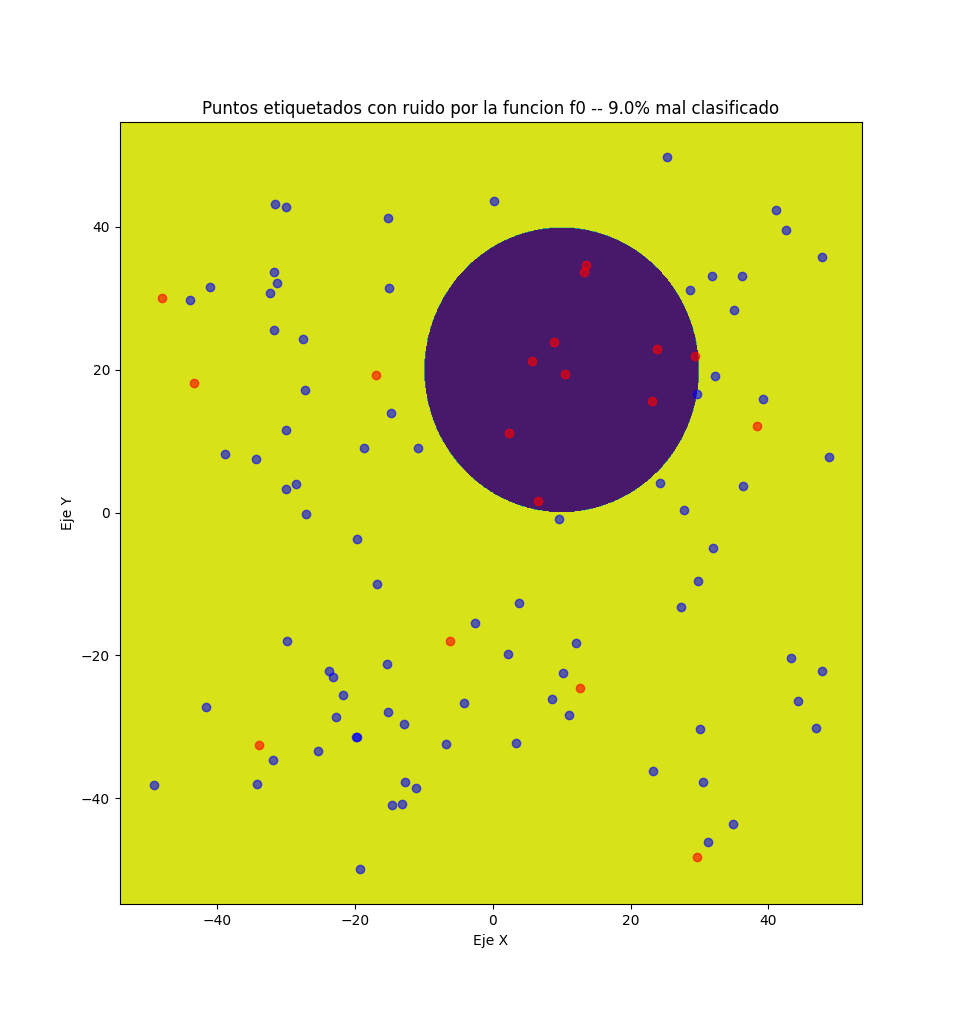
\includegraphics[width=0.60 \textwidth]{puntos_clasificados_experimento_f0.png}
    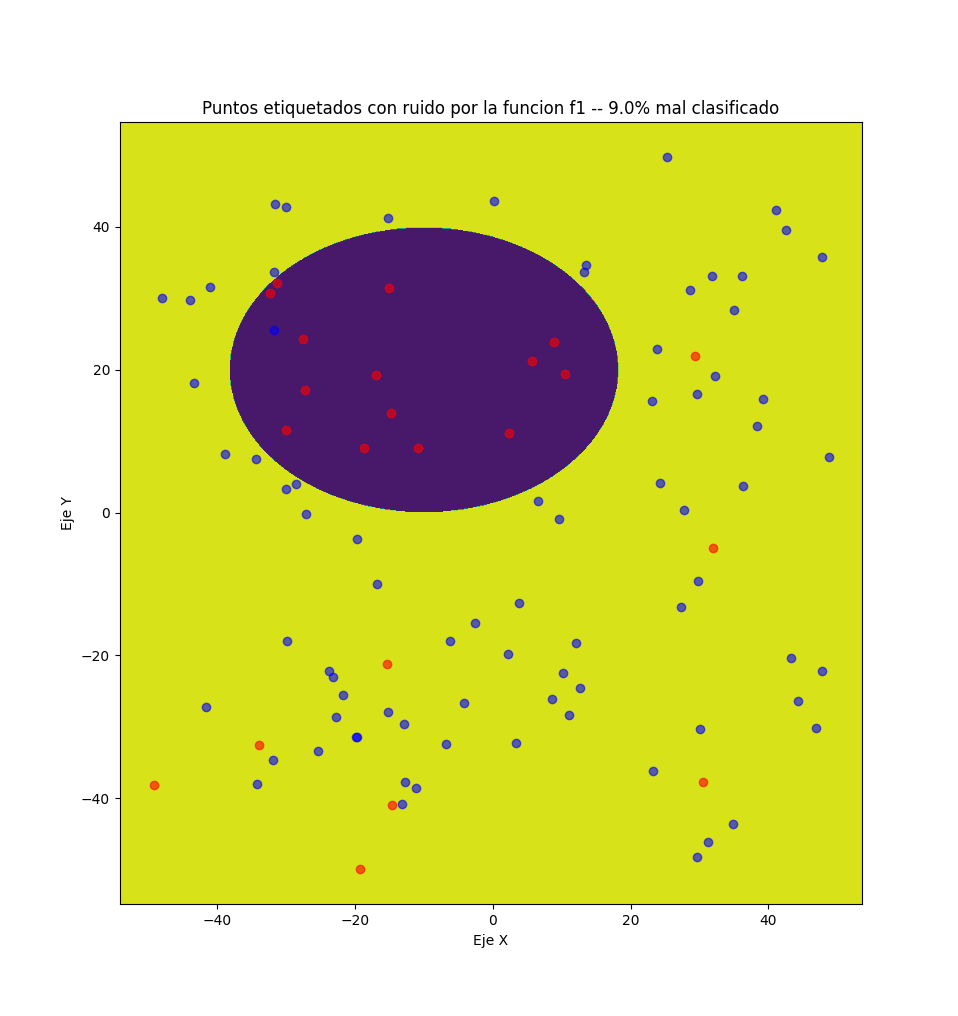
\includegraphics[width=0.60 \textwidth]{puntos_clasificados_experimento_f1.png}

    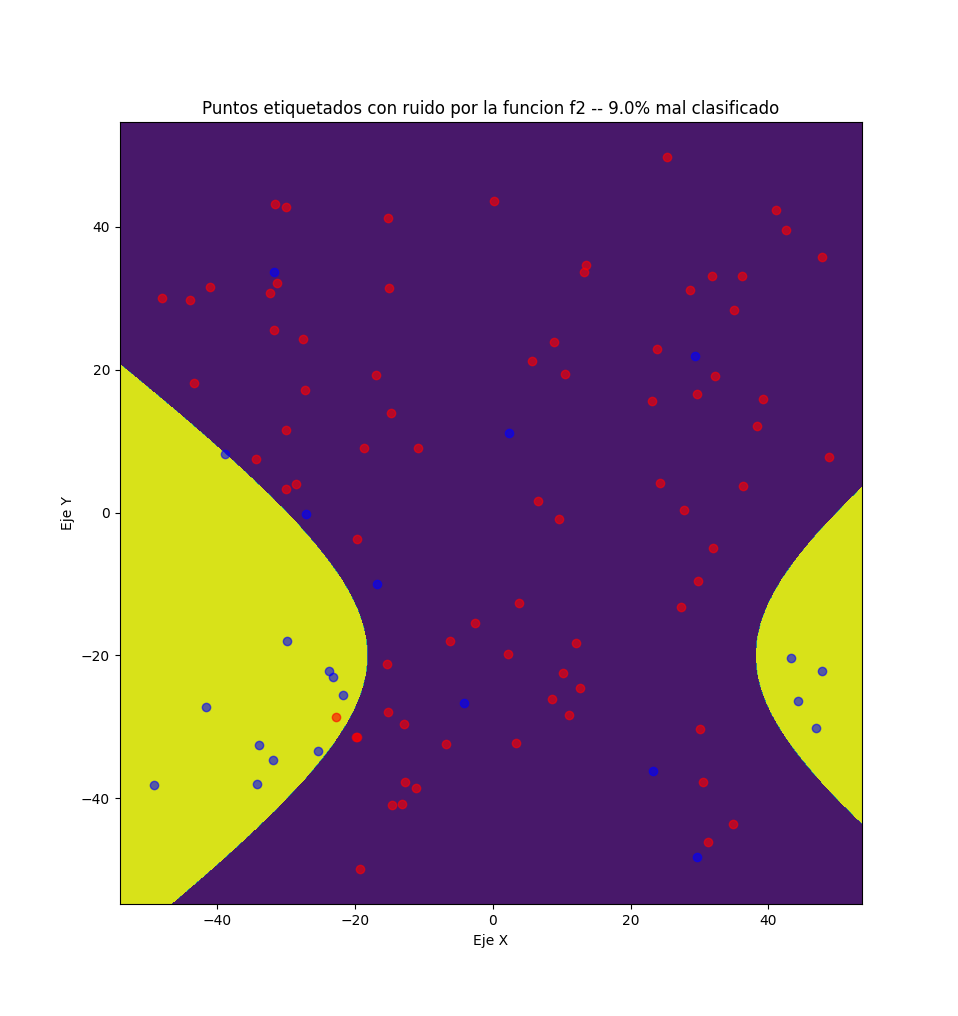
\includegraphics[width=0.60 \textwidth]{puntos_clasificados_experimento_f2.png}
    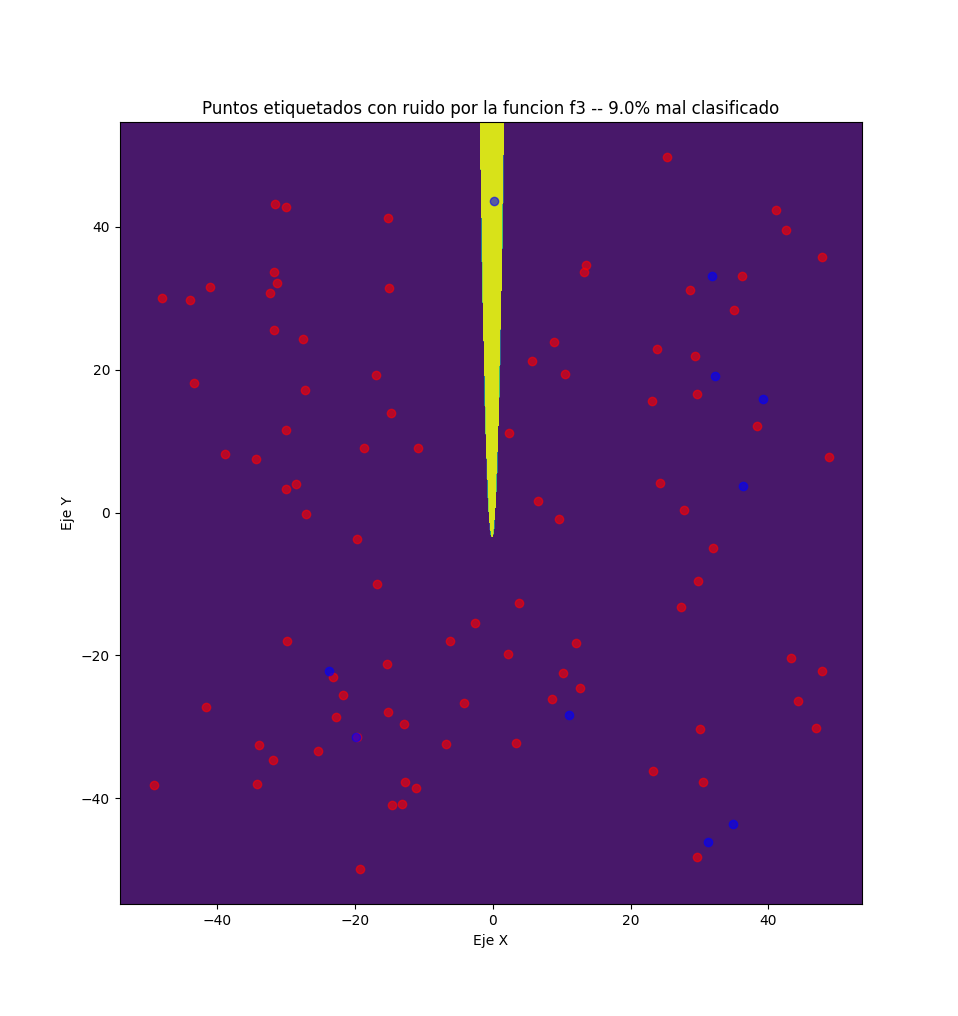
\includegraphics[width=0.60 \textwidth]{puntos_clasificados_experimento_f3.png}

    \caption{Etiquetado ruidoso con las cuatro funciones dadas}
\end{figure}

Comenzamos valorando la complejidad aparente de las funciones. Toda esta discusión es desde un punto de vista intuitivo. Pero no estamos cuantificando estas nociones, pudiendo llegar a ser falaz. Por tanto, después de este análisis superficial, realizamos un análisis más profundo y cuantitativo.

Es claro que la recta realiza una clasificación mucho más sencilla que estas nuevas funciones de clasificación, pues divide el espacio en dos regiones sencillas: la región por encima de la recta y la región por debajo de la recta. $f_0$ ya es más compleja pues estamos considerando la región fuera y dentro de un círculo, que no está centrado en el origen. $f_1$ es algo más compleja, pues ahora no consideramos un círculo, sino una elipse (añadimos un nuevo parámetro al modelo, el achatamiento del eje $x$ dado por el factor $\frac{1}{a^2}$). En $f_2$ estamos considerando regiones hiperbólicas, que viene determinada por el mismo número de parámetros que $f_1$, aunque la forma de las regiones cambie al cambiar la cónica cambiando el signo. Y en este caso, hay un predominio de región de etiquetado positivo frente a la región de etiquetado negativo. Y finalmente en $f_3$ consideramos una parábola, cuya región de etiquetado negativo tiene un área muy pequeña comparada a la región de etiquetado positivo.

Bajo estas condiciones es algo complicado comentar si estas funciones más complejas son mejores clasificadores que la función lineal, pues esto dependerá de una serie de factores.

Pasamos a valorar la complejida de las funciones de una forma objetiva, cuantitativa, y teniendo en cuenta la muestra de datos con la que estamos trabajando.

Para empezar, estamos trabajando con 100 puntos o datos. Debemos emplear algún método para concer si la complejidad de nuestras funciones se adecúa a la cantidad de datos con los que estamos trabajando. Esta herramienta será la \textbf{dimensión de Vapnik-Chervonenkis}. Sabemos que en el caso de la recta, $d_{VC} = d + 1 = 3$, y por tanto, la regla práctica para generalizar bien $N \geq 10 d_{VC}$ se cumple. Para el caso del círculo y de la elipse, tenemos también que $d_{VC} = 3$. Esto no es difícil de probar, al tener una dimensión tan baja, con ejemplos \footnotemark. Por tanto, a nivel de generalización, con los 100 datos que tenemos es suficiente pues $100 \geq 3 * 10$. Para el caso de la hipérbola y de la parábola hemos comprobado que $d_{VC} = 3$ yendo ejemplo por ejemplo (puede estar mal hecho el cálculo). Por lo cual, todas las funciones tienen una cantidad suficiente de datos acorde a $d_{VC}$ como para que no haya problemas para generalizar (siempre siguiendo la regla práctica $N \geq d_{VC} * 10$).
\footnotetext{En \cite{PowerPoi66:online} se muestra de forma visual la prueba de esto con los conjuntos dados de datos. En \cite{machinel96:online} se realiza una prueba formal de este hecho.}

Sería más adecuado realizar experimentos con un dataset de entrenamiento y otro de test para comprobar empíricamente que, efectivamente, con 100 datos no tenemos problemas de generalización.

Notar que la función lineal sigue siendo más sencilla aunque $d_{VC}$ parezca indicar lo contrario. Esto se debe a que en el análisis \emph{VC}, nos situamos en el peor de los casos, es un análisis muy pesimista.

Otro punto a tener en cuenta es el problema que estamos considerando. Sigue sin tener demasiado sentido plantearse el clasificado en abstracto y comparar lo bueno que son los clasificadores desde este punto de vista. Si las características del problema tienen un carácter lineal (al doble de ingresos, el doble de probabilidad de que nos acepten la solicitud de un crédito, por ejemplo), las funciones de clasificado no lineales no tienen demasiado sentido. Si por otro lado las características de los datos no son lineales, entonces puede tener más sentido usar clasificadores no lineales a pesar de que representen un modelo más complejo, pues serían más correctos desde la perspectiva del problema a resolver.

Respecto al proceso de modificación de etiquetas, las condiciones en la que hemos realizado este proceso también complica algo las cosas. Hemos modificado, aleatoriamente, un 10\% de las etiquetas positivas y otro 10\% de las etiquetas negativas. En este proceso da bastante igual la forma que tome $f$. En el sentido en el que, podemos pensar que la recta es muy robusta frente al ruido, o más robusta que una elipse. Pero a la hora de ejecutar el cambio aleatorio, esto no se tiene en cuenta.

Esto se refleja en que obtenemos constantemente un error del 9\%. Que no sea un 10\% puede ser por la cantidad de etiquetas negativas y positivas. Al no ser numeros que al multiplicarlos por $0.1$ den un entero, se puede redondear por la baja, obteniendo así este error porcentual algo más bajo que el 10\%.

Sin embargo, si que hemos detectado una característica en la que la forma de $f$ influye en el proceso. Esto se ve claro con $f_3$. Al tener una región mucho más pequeña que la contraria (en este caso, región de etiquetado negativo mucho más pequeña que la región de etiqetado positivo), es muy probable que no hayamos clasificado ningún punto como negativo, y por tanto realizamos modificaciones del tipo $negativo \rightarrow positivo$, solo modificaciones del tipo $positivo \rightarrow negativo$. Aún así, esto no es demasiado relevante

Así queda justificado que el proceso de introducción de ruido no es muy informativo. Un proceso de introducción de ruido mucho más interesante podría haber sido seleccionar aleatoriamente un porcentaje de las etiquetas, tanto positivas como negativas, y en vez de cambiar arbitrariamente su etiqueta, modificar en un cierto rango acotado su posición, y ver si en esa nueva posición se etiquetaría con el otro valor.

Esto nos daría más información sobre la robustez de nuestro clasificador frente al ruido. Por ejemplo, en el caso de la recta, un punto alejado de la frontera no cambiaría de etiqueta (con un rango de variación de coordenadas razonable), mientras que un punto muy cercano a la frontera sí que cambiaría. Como se puede ver en la imagen, la mayoría de puntos no se encuentran muy pegados a la frontera. Por otro lado, considerando $f_3$, podríamos pensar que todos los puntos de etiquetado negativo se saldrían de la región de etiquetado negativo, al ser esta muy estrecha, concluyendo que el clasificador es muy frágil frente al ruido.

Otra forma de medir esta \emph{robustez} sería calcular la longitud de las fronteras de nuestro clasificador. A mayor longitud, tenemos un modelo más complejo, que es más probable de sobreajustar. Además, a mayor longitud es más probable que un cambio de coordenadas aleatoria, anteriormente discutida, provoque un cambio de etiqueta. Y por tanto es más probable que el ruido afecte a nuestro problema.

Resumiendo, consideramos insuficiente la información dada para comparar las funciones de clasificación. Por tanto, realizamos nuevas consideraciones para tratar de realizar un mejor análisis, y proponemos una forma sintética de introducir ruido que pensamos que puede ser más adecuada a la hora de analizar la robustez de los clasificadores frente al ruido.

\pagebreak

\section{Ejercicio 2 - Modelos lineales}

% TODO -- incluir el pseudocodigo
La función \lstinline{ajusta_PLA(datos, label, max_iter, vini)} está implementada bajo el nombre \lstinline{perceptron_learning_algorithm}. Esta función recibe los parámetros indicados por el guión, y uno adicional. Este parámetro adicional es el booleano \lstinline{verbose}, que cuando se pasa como \lstinline{True}, devuelve la solución, las iteraciones consumidas y el error porcentual en la muestra de cada iteración. Cuando es \lstinline{False}, solo devolvemos la solución y el número de iteraciones consumidas. Notar que las iteraciones consumidas se corresponden con la cantidad de \emph{Epochs} consumidos (pasadas completas sobre todo el conjunto de datos). El error por cada iteración también se refiere al error por cada \emph{Epoch}. El algoritmo es tan sencillo que no parece necesario incluir el pseudo-código. Además, la implementación es también muy directa, por lo que no parece necesario hacer aclaraciones sobre decisiones tomadas para implementar el algoritmo.

\subsection{Apartado a) - Algoritmo Perceptron}

Ejecutamos el algoritmo \emph{PLA} sobre los datos generados en \ref{section:ejercicio1.2.a}. Recordemos que estos datos han sido clasificados por una recta aleatoria, sin introducir todavía error. Por lo tanto, son claramente linealmente separables, y por ello, el algoritmo deberá alcanzar una solución en un número finito de iteraciones, con un error dentro de la muestra del $0.0\%$.

\subsubsection{Subapartado 1}

Para usar los mismos datos que en \ref{section:ejercicio1.2.a}, usamos variables globlales para guardar en ese primer ejercicio los datos generados. Otra observación pertinente es que a la función \lstinline{perceptron_learning_algorithm} le tenemos que pasar un número máximo de iteraciones. Queremos alcanzar la solución antes de agotar las iteraciones, porque sabemos que la muestra es linealmente separable. Por tanto hacemos una asignación lo suficientemente grande: \lstinline{max_iterations = 5000}.

Mostramos de nuevo la gráfica de los datos etiquetados para asegurarnos de que estamos en el mismo ambiente que en \ref{section:ejercicio1.2.a}:

\begin{figure}[H]
    \centering
    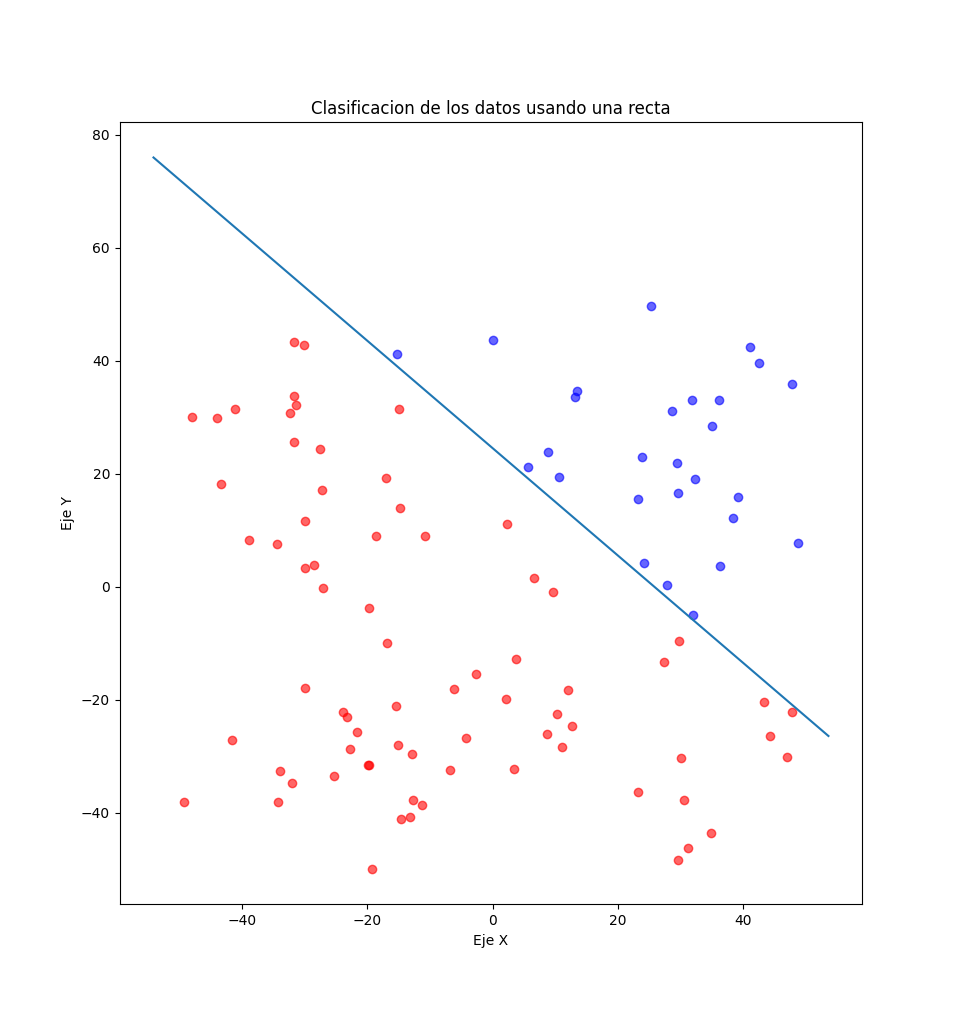
\includegraphics[scale=0.3]{puntos_clasificados_recta02}
    \caption{Datos clasificados por la recta aleatoria}
\end{figure}

Lanzamos 10 veces el algoritmo para el vector inicial cero, y otras 10 para vector inicial aleatorio y mostramos los resultados del experimento por pantalla:

\begin{lstlisting}[caption={Resultados para vector inicial cero}, captionpos=b]
Resultado de las 10 iteraciones -- Vector Inicial Cero:
-> Errores finales(tanto por uno): [0.0, 0.0, 0.0, 0.0, 0.0,
                                    0.0, 0.0, 0.0, 0.0, 0.0]
-> Valor medio de los errores: 0.0%
-> Desviacion tipica de los errores: 0.0
-> Iteraciones consumidas: [63, 49, 27, 52, 45, 28, 13, 60, 39, 39]
-> Valor medio de iteraciones: 41.5
-> Desviacion tipica del numero de iteraciones: 14.8340
\end{lstlisting}

\begin{lstlisting}[caption={Resultados para vector inicial aleatorio} ,captionpos=b]
Resultado de las 10 iteraciones -- Vector Inicial aleatorio:
-> Errores finales(tanto por uno): [0.0, 0.0, 0.0, 0.0, 0.0,
                                    0.0, 0.0, 0.0, 0.0, 0.0]
-> Valor medio de los errores: 0.0%
-> Desviacion tipica de los errores: 0.0
-> Iteraciones consumidas: [120, 78, 26, 25, 47, 27, 42, 44, 44, 13]
-> Valor medio de iteraciones: 46.6
-> Desviacion tipica del numero de iteraciones: 29.6856
\end{lstlisting}

Ambos algoritmos, como era de esperar, convergen a una solución de error $E_{in} = 0.0\%$. Por lo tanto, no merece hacer comparaciones sobre los errores alcanzados. Sin embargo, las iteraciones necesarias para converger sí que son distintas. Para el vector inicial cero, tenemos un menor número medio necesario de iteraciones necesarias que con vector inicial aleatorio, aunque la diferencia no es demasiado grande. Además, la desviación típica del número necesario de iteraciones para converger es menor usando el vector inicial cero que en el vector inicial aleatorio. Era de esperar pues al inicializar de forma aleatoria estamos introduciendo mucha más variabilidad al algoritmo. Por tanto, el vector inicial cero resulta más adecuado en este ambiente: requiere en media menos iteraciones y es más estable respecto a dicho número necesario de iteraciones.

También mostramos los gráficos de convergencia para una ejecución de \emph{PLA} con vector inicial cero, y otro para vector inicial aleatorio:

\begin{figure}[H]
    \begin{subfigure}{0.3\textwidth}
        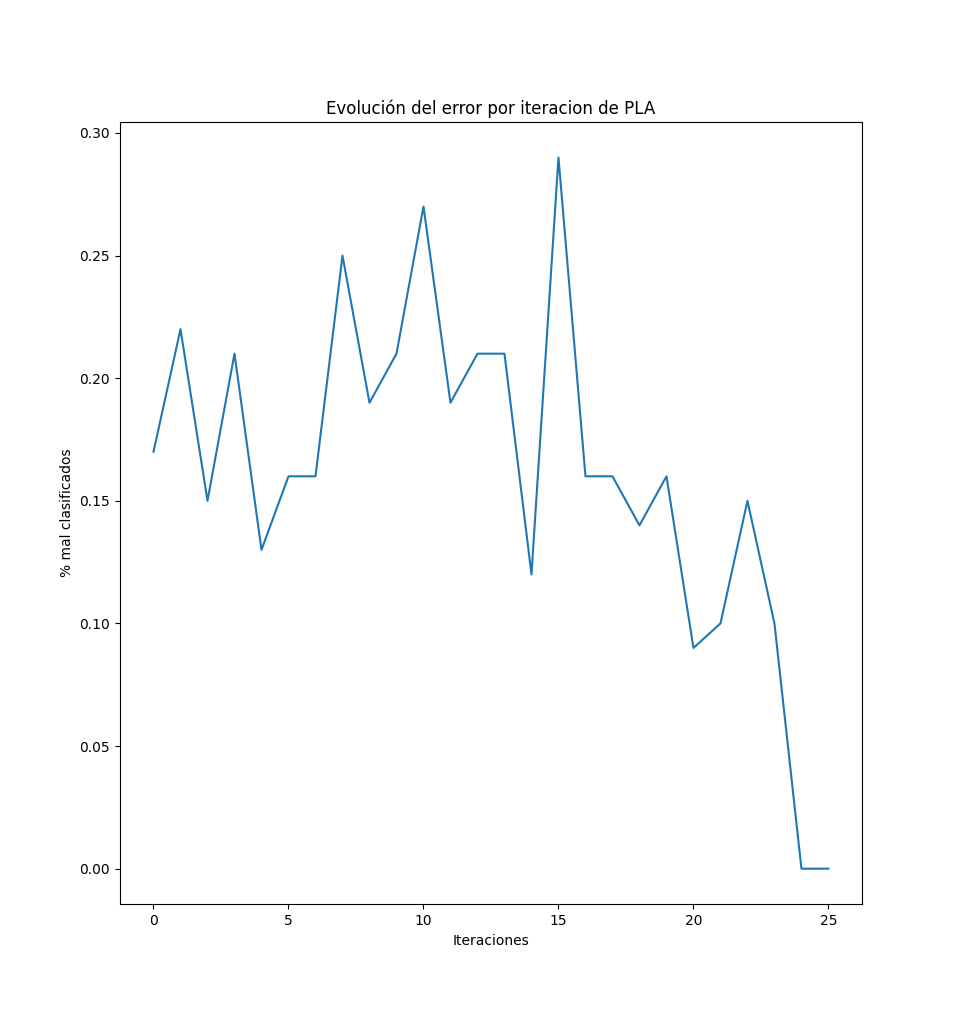
\includegraphics[scale=0.3]{grafica_convergencia_pla_cero}
        \caption{$V_{ini}$ inicial cero}
    \end{subfigure} \hspace{0.2\textwidth}
    \begin{subfigure}{0.3\textwidth}
        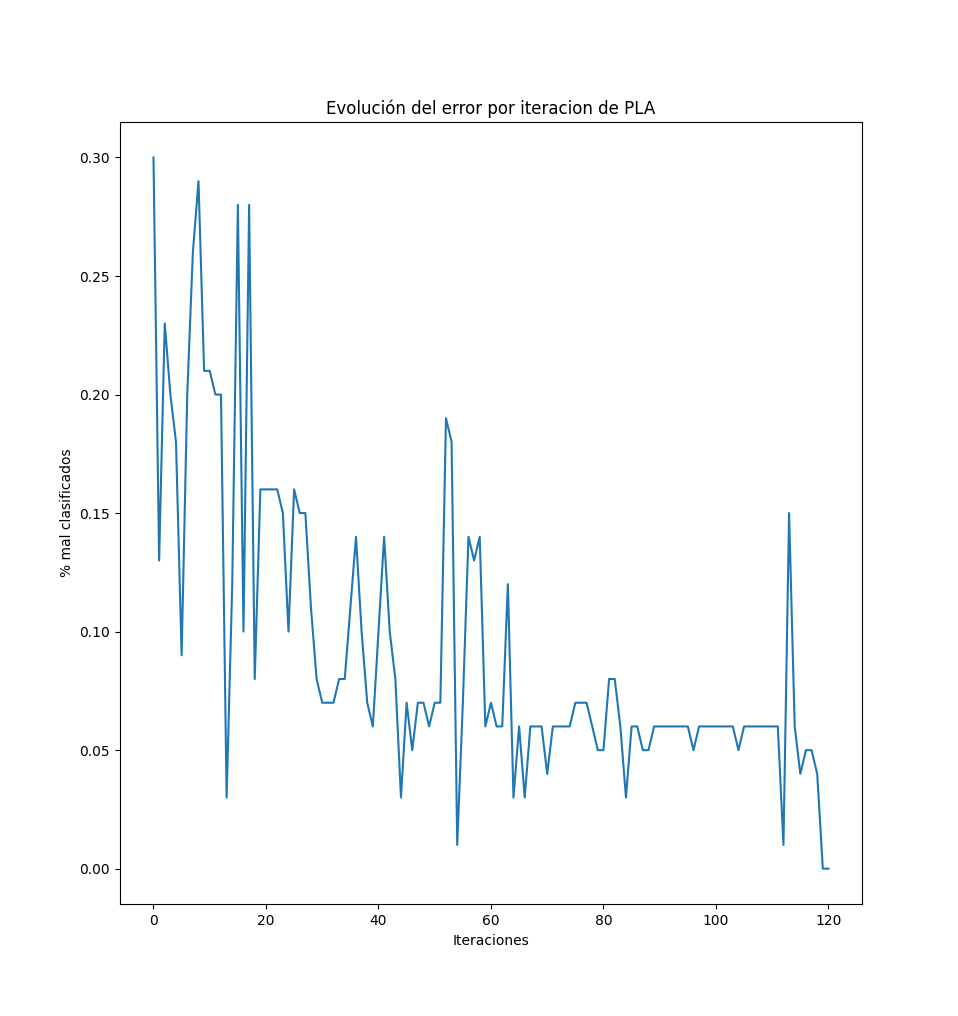
\includegraphics[scale=0.3]{grafica_convergencia_pla_aleatorio}
        \caption{$V_{ini}$ aleatorio}
    \end{subfigure}
    \caption{Gráficas de convergencia para PLA}
\end{figure}

Con estos gráficos podemos pensar que el vector inicial cero es mucho más rápido en converger, y mucho más estable que el vector inicial aleatorio. Pero con los 10 experimentos hemos visto que no es demasiado más rápido, aunque si que es bastante más estable entre distintas ejecuciones (aquí el aleatorio ha tenido una ejecución muy mala, lo cual es probable al tener una desviación típica alta).



\subsubsection{Subapartado 2}

Repetimos el mismo experimento pero usando ahora los datos con ruido, generados en \ref{section:ejercicio1.2.b}. De nuevo, para conseguir esto, lo que hacemos es guardar las etiquetas ruidosas en una variable global, y reusarlas aquí. De nuevo, mostramos la gráfica de etiquetado ruidoso para asegurarnos de que estamos trabajando con los mismos datos que en \ref{section:ejercicio1.2.b}:

\begin{figure}[H]
    \centering
    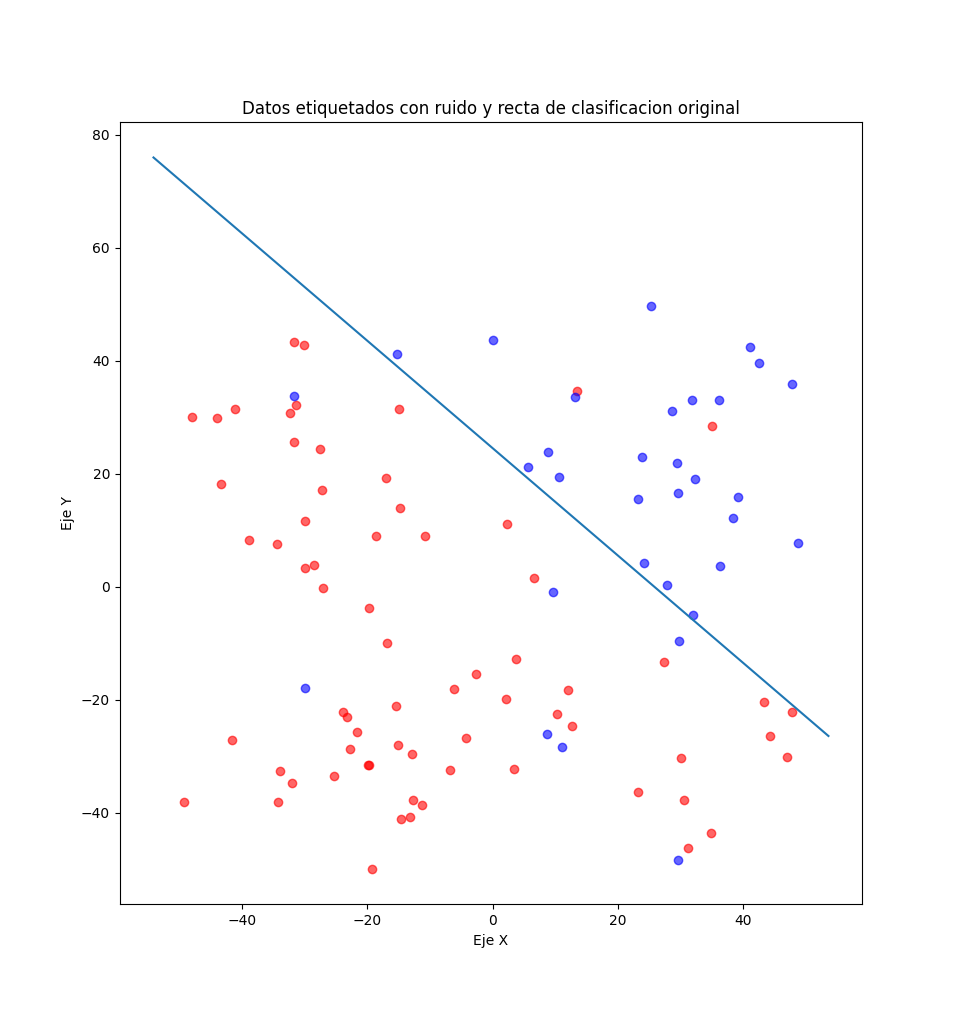
\includegraphics[scale=0.3]{puntos_clasificados_recta_aleatorizados02}
    \caption{Datos clasificados por la recta aleatoria con ruido sintético}
\end{figure}

Y de nuevo, mostramos los resultados del experimento:

\begin{lstlisting}[caption={Resultados para vector inicial cero y ruido en las etiquetas}, captionpos=b]
Resultado de las 10 iteraciones -- Vector Inicial Cero:
-> Errores finales(tanto por uno): [0.19, 0.2, 0.17, 0.09, 0.2,
                                    0.17, 0.18, 0.13, 0.09, 0.28]
-> Valor medio de los errores: 17.0%
-> Desviacion tipica de los errores: 0.0536
-> Iteraciones consumidas: [5000, 5000, 5000, 5000, 5000, 5000, 5000, 5000, 5000, 5000]
-> Valor medio de iteraciones: 5000.0
-> Desviacion tipica del numero de iteraciones: 0.0
\end{lstlisting}


\begin{lstlisting}[caption={Resultados para vector inicial aleatorio y ruido en las etiquetas}, captionpos=b]
Resultado de las 10 iteraciones -- Vector inicial aleatorio:
-> Errores finales(tanto por uno): [0.2, 0.26, 0.09, 0.29, 0.17,
                                    0.26, 0.18, 0.13, 0.1, 0.27]
-> Valor medio de los errores: 19.5%
-> Desviacion tipica de los errores: 0.0694
-> Iteraciones consumidas: [5000, 5000, 5000, 5000, 5000, 5000, 5000, 5000, 5000, 5000]
-> Valor medio de iteraciones: 5000.0
-> Desviacion tipica del numero de iteraciones: 0.0
\end{lstlisting}

En este caso, los datos no son linealmente separables por el ruido, y por lo tanto, \emph{PLA} no convergerá. Por lo cual, el algoritmo consumirá el número máximo de iteraciones, el cual está establecido a un valor de $5000$. Teniendo en cuenta que anteriormente necesitábamos de media aproximadamente 40-45 iteraciones sobre \emph{Epochs}, este valor de $5000$ parece más que razonable para ajustarnos a la muestra.

Al consumir ambos el máximo de iteraciones, no podemos realizar comparaciones respecto a esto entre los dos algoritmos. Con vector inicial cero hemos obtenido un error ligeramente mejor que con vector inicial aleatorio. Además, la desviación típica de los errores es menor, por lo que nos encontramos con que el vector inicial cero proporciona en media errores más bajos y es más estable que considerar vector inicial aleatorio. Y de nuevo, como en el caso de un \emph{dataset} linealmente separable, concluimos que es mejor considerar un vector inicial cero que un vector inicial aleatorio.

Al igual que hacíamos en el subapartado anterior, mostramos la gráfica de convergencia. Con la diferencia de que esta vez, solo mostramos la ejecución para vector inicial aleatorio.

\begin{figure}[H]
    \centering
    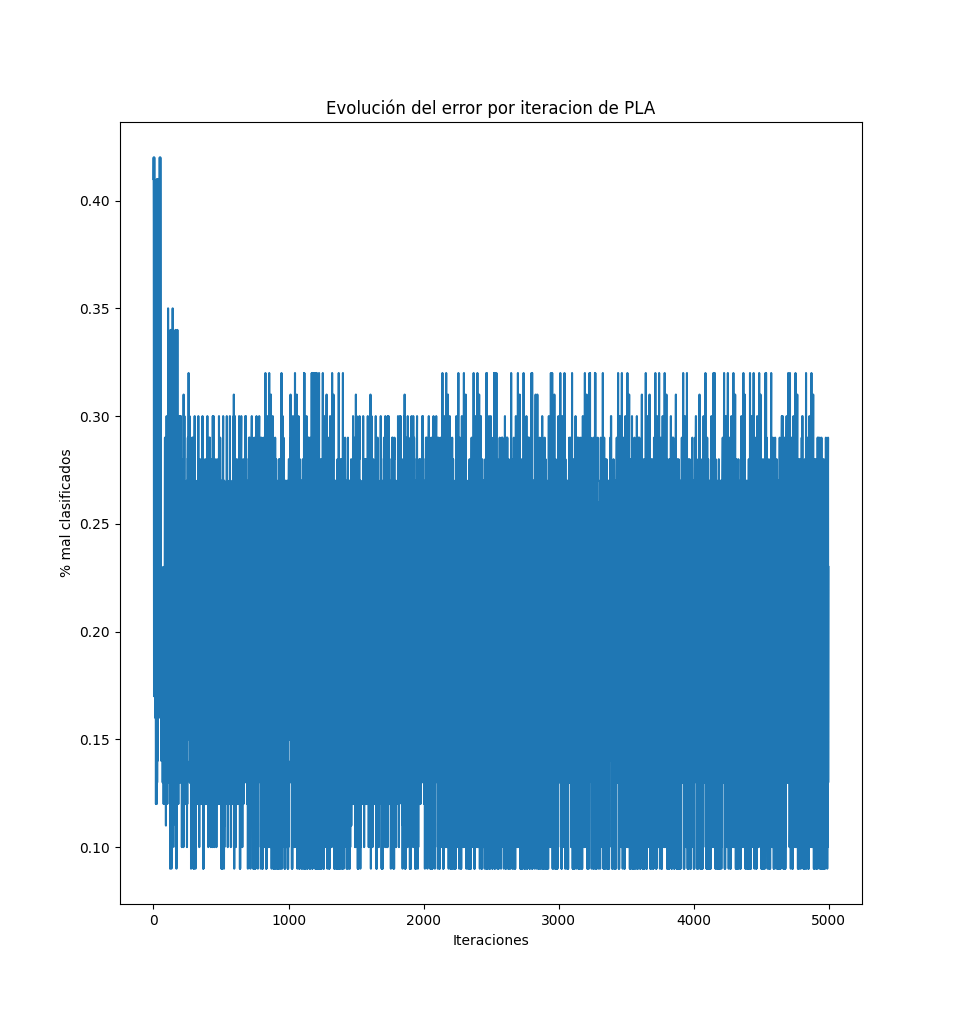
\includegraphics[scale=0.4]{grafica_convergencia_pla_ruido_cero}
    \caption{Gráfica de convergencia - PLA con $V_{ini} = 0$ y ruido sintético}
\end{figure}

Se ve claramente el comportamiento errático de \emph{PLA} que conocíamos de teoría. Por tanto, no tiene sentido que mostremos otro gráfico viendo el progreso usando vector inicial aleatorio. Este gráfico es útil para ver que, aunque con el experimento digamos que usando vector inicial cero tenemos más estabilidad que usando vector inicial aleatorio, la estabilidad del algoritmo en general es muy mala. Además, motiva el uso de la mejora \emph{PLA-Pocket}. Usando esta mejora del algoritmo, obtendríamos una gráfica de convergencia monótonamente decreciente.

Además, queda claro que 5000 iteraciones son más que suficientes, pues nunca vamos a lograr $E_{in} = 0$, y además, al no decrecer el error monótonamente tampoco parece beneficioso consumir más iteraciones.

\pagebreak
\subsection{Apartado b) - Regresión logística}

Empezamos esta sección explicando cómo vamos a generar nuestra muestra de datos. Tenemos una población hipotética $\chi = [0, 2] \times [0, 2]$ y la probabilida de tomar un $x \in \chi$ es uniforme. Por tanto, para generar tanto las muestras de entrenamiento como de test, lo que hacemos es invocar a una función que nos da un punto aletorio con probabilidad uniforme en ese intervalo bidimensional.

La función \lstinline{generate_dataset} toma un número dado de puntos aleatorios en $\chi$. Usaremos esta función tanto para las muestras de entrenamiento como para las de test.

Para generar la recta aleatoria de etiquetado, tomamos dos puntos aleatorios (con \lstinline{generate_dataset(2)}) y calculamos la recta que pasa por esos dos puntos con \lstinline{calculate_straight_line_from_two_points}.

En regresión logística, usamos la siguiente función de etiquetado:

$$
f_w(x):= \left\{ \begin{array}{lcc}
        1 &  si & \sigma(signal) \geq 0.5 \\
    \\ -1 &  si & \sigma(signal) < 0.5
    \end{array}
\right.
$$

donde $\sigma(x) := \frac{1}{1 + e^{-x}}$ y $signal$ es la señal lineal dada por $signal := w^T x$. Es claro que lo que aprendemos de este modelo son los valores de los pesos: $w$.

Antes de realizar el experimento 100 veces, vamos a ejecutar una repetición del experimento, mostrando ciertas gráficas y realizando algunos análisis antes de realizar. Tras esto, lanzamos 100 veces el experimento, obteniendo más información para realizar los análisis.

\subsubsection{Regresión logística con Gradiente Descendente Estocástico}

La primera consideración para implementar regresión logística junto a gradiente descendente estocástico es la necesidad de añadir una columna de unos a la matriz de datos. Esta columna en la primera práctica ya venía dada. Pero en este caso, necesitamos añadirla manualmente. Esta columna representa el término independiente de la combinación lineal que subyace al modelo lineal. Podríamos hacerlo sin esta columna, pero en ese caso no podemos fijar un \emph{offset} a los datos. Para añadir la columna de unos disponemos de la función \lstinline{add_colum_of_ones}.

El algortimo de gradiente descendente estocástico ya fue explicado en la anterior práctica. Todas las consideraciones sobre la implementación de este algoritmo ya fueron expuestas en la anterior memoria (por ejemplo, la generación de \emph{minibatches} mezclados aleatoriamente de forma eficiente y cómoda). Así que para este problema, tenemos que realizar las siguientes modificaciones:

\begin{itemize}
    \item El error que consideramos viene dado por $E_{in} = \frac{1}{N} \sum ln(1 + e^{-y_i w^T x_i})$. Este es el error que vamos a mostrar en las gráficas de convergencia.
    \item Por tanto, para el gradiente usamos la expresión $\nabla E_{in} = -\frac{1}{N} \sum \frac{y_n x_n}{1+e^{y_n w^T x_n}}$
    \item La solución inicial será un vector de ceros
    \item La condición de parada será $||w(t+1) - w(t)|| \leq 0.01$
    \item Learning rate $\eta = 0.01$
\end{itemize}

Al tener una condición distinta de parada, dejamos el número máximo de iteraciones a \lstinline{None}, para iterar hasta que tengamos la distancia entre dos soluciones consecutivas por debajo de la cota dada.

Otro aspecto crítico es establecer el \emph{batch size}. El guión nos indica que debemos usar un \lstinline{batch size = 1}, pero realizamos una corta exploración sobre distintos valores. Con un valor de 1, necesitamos muchas iteraciones pero llegamos a un muy buen error, aproximadamente en $[0.005 - 0.01]$ según la semilla aleatoria. Para \lstinline{batch_size = 4}, requerimos entre 1500 - 5000 iteraciones, pero el error pasa a estar en $[0.01 - 0.05]$. A partir de \lstinline{batch_size = 8}, tenemos muy pocas iteraciones (por debajo de 1000), pero con un error por encima de $0.2$. Por tanto, hemos comprobado de forma empírica y rápida que el valor adecuado para \lstinline{batch_size} es 1. No tenemos mucha intuición por lo que esto es así. Una hipótesis es que, al estar en un problema de clasificación, lo adecuado es visitar punto a punto e ir ajustando localmente con la información de ese punto. Este es un esquema parecido a \emph{PLA}, donde visitamos punto a punto y ajustamos si hemos fallado en ese punto. Además, al estar considerando solo la condición de distancia entre soluciones consecutivas, con $batch\_size > 1$ puede ser que acabemos compensando la dirección del error entre los múltiples puntos (por ejemplo, errores con la misma dirección pero distinto sentido), provocando una parada prematura. Intuimos por tanto que estableciendo otras condiciones de parada (como que el error esté por debajo de cierta cota) puede funcionar mejor si queremos establecer un $batch\_size  >1$. Esta última idea se refuerza más adelante, cuando vemos que la muestra de datos es linealmente separable, por lo que deberíamos ser capaces de alcanzar error 0.0\% en la muestra, iterando el suficiente número de veces.

\subsubsection{Conjunto de datos con el que trabajamos} \label{section:conjunto_datos_lgr}

Generamos el conjunto de datos, de la forma que ya hemos comentado:

\begin{figure}[H]
    \centering
    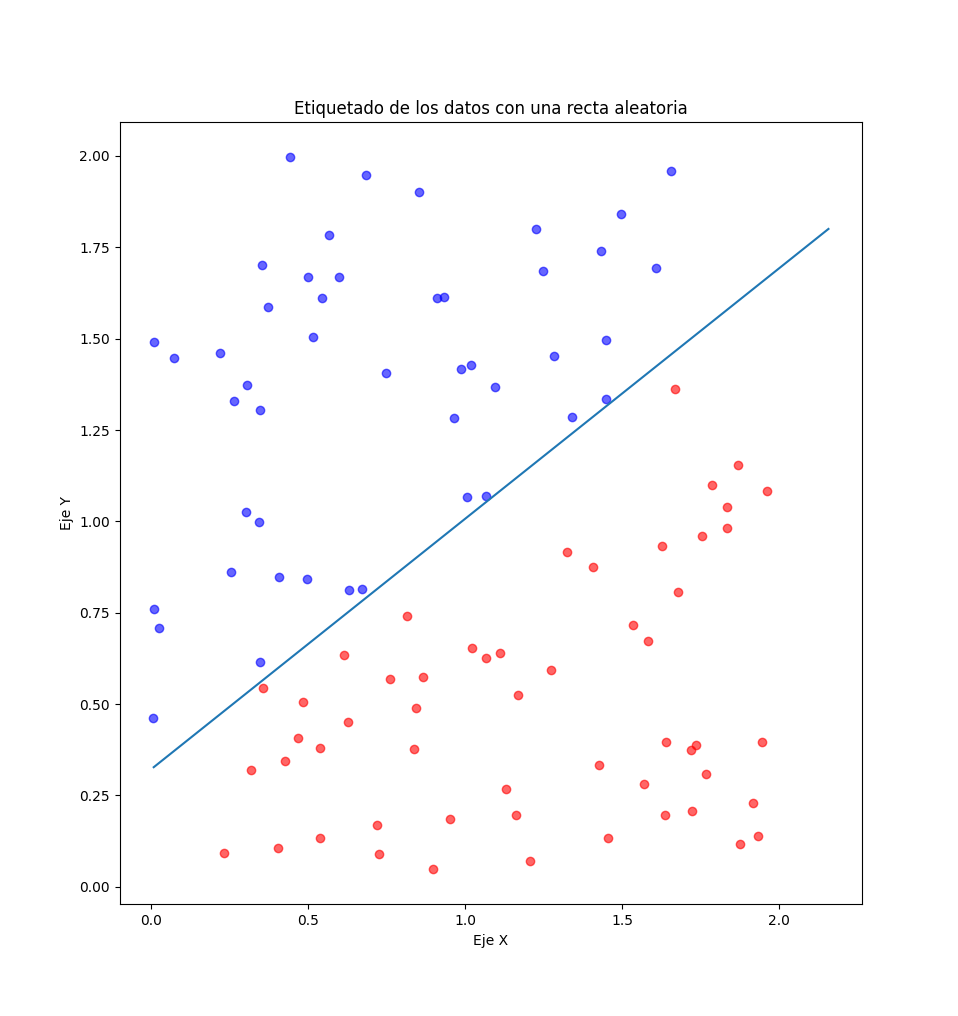
\includegraphics[width = 0.5\textwidth]{muestra_datos_lgr}
    \caption{Muestra de datos etiquetada por la recta aleatoria}
\end{figure}

Claramente el proceso de etiquetado hace que la muestra de datos linealmente separable. Por tanto, es de esperar que regresión logística con gradiente descendente estocástico alcance un $E_{in} = 0.0\%$.

\subsubsection{Entrenamiento y resultados}

Al lanzar \emph{LGR} con \emph{SGD} obtenemos la siguiente salida por pantalla:

\begin{lstlisting}[caption={Resultados del entrenamiento}, captionpos=b]

- Pesos obtenidos: [-2.57253883 -4.89587868  7.85922036]
- Iteraciones consumidas: 34600
- Error final alcanzado (error LGR): 1.1013766997935295
- Error final alcanzado (porcentaje mal clasificado): 0.0%

\end{lstlisting}

Los resultados obtenidos eran los que esperábamos. El error \emph{cross-entropy} no se anula, mientras que el porcentaje de puntos mal clasificados es cero. Mostramos la gráfica de convergencia:

\begin{figure}[H]
    \begin{subfigure}{0.4\textwidth}
        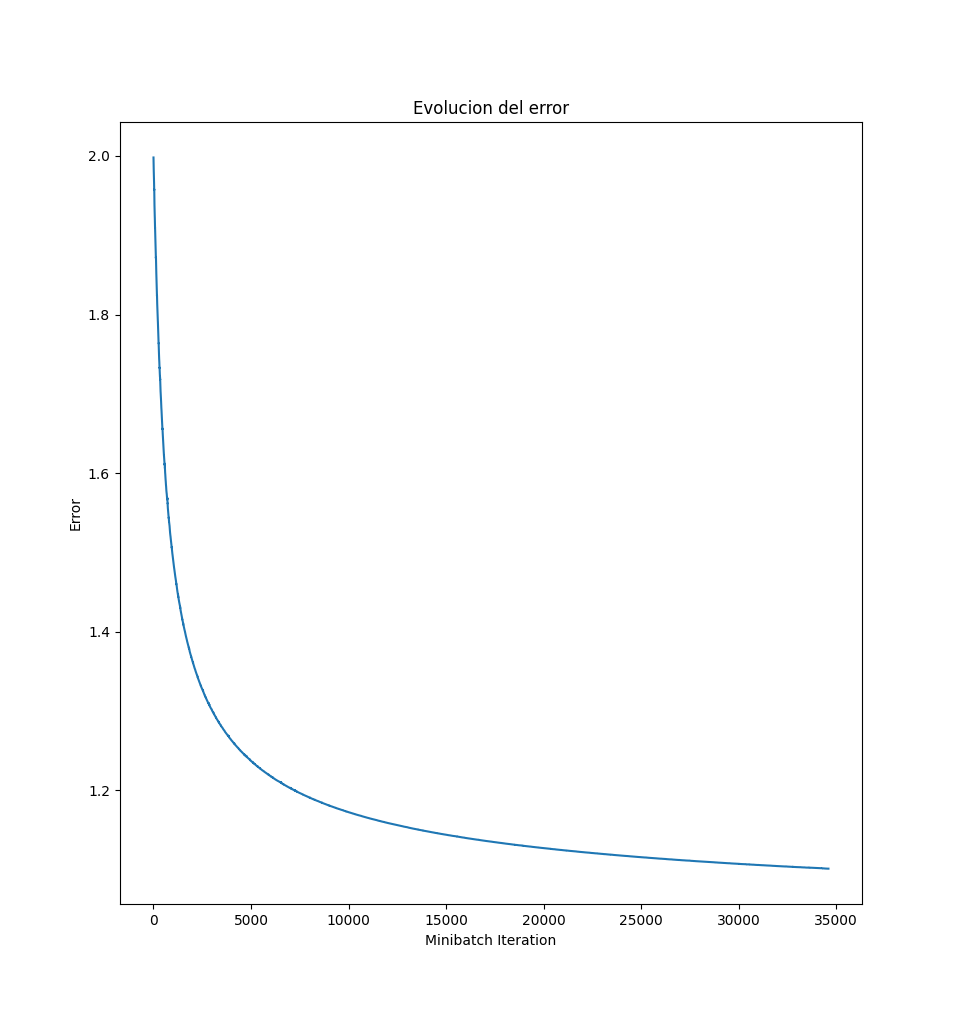
\includegraphics[scale=0.3]{grafica_convergencia_lgr}
        \caption{Gráfica de convergencia}
        \label{figure:sin_ampliar}
    \end{subfigure} \hspace{0.2\textwidth}
    \begin{subfigure}{0.4\textwidth}
        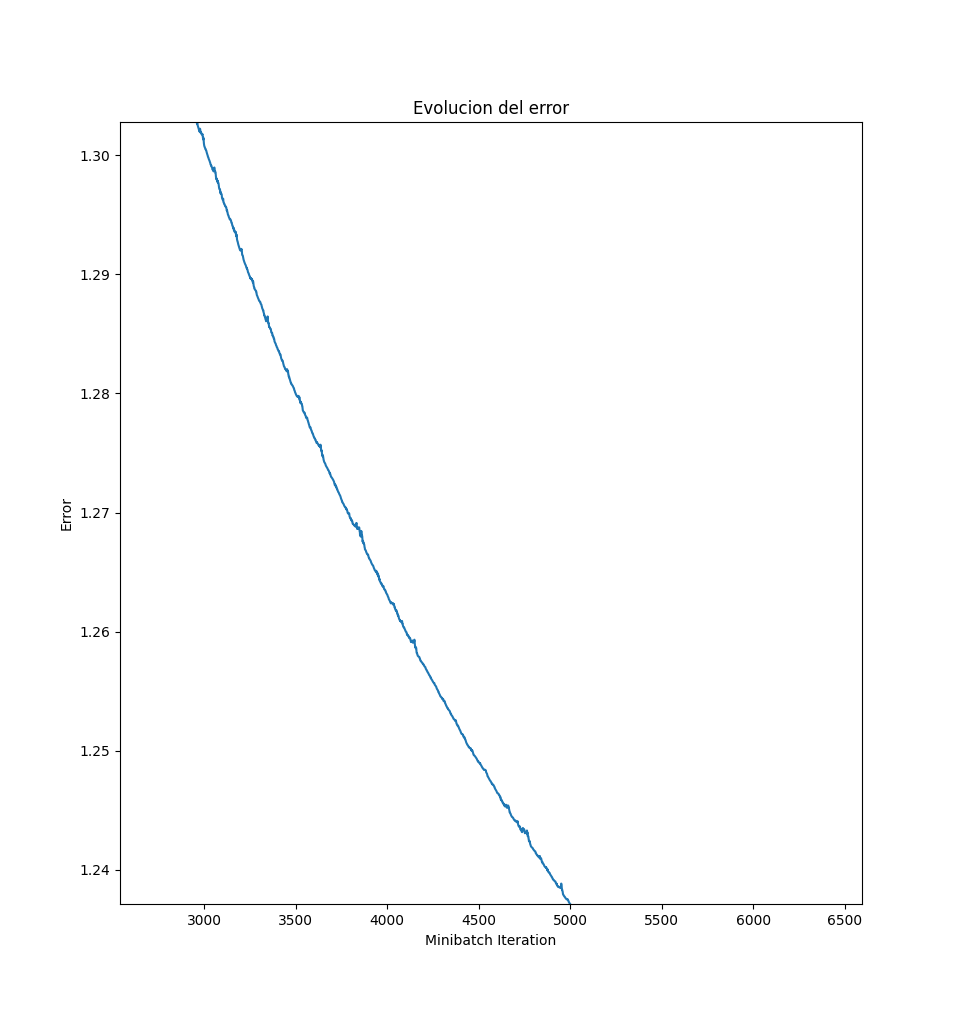
\includegraphics[scale=0.3]{grafica_convergencia_lgr_zoom}
        \caption{Gráfica de convergencia ampliada}
    \end{subfigure}
    \caption{Gráficas de convergencia para LGR-SGD}
\end{figure}

Vemos que el comportamiento del gradiente descendiente es adecuado. Pareciera que en \ref{figure:sin_ampliar} tenemos convergencia monótona. Por eso mostramos un \emph{"zoom"} de la gráfica para ver que no es así, como es lo normal cuando usamos minibatches para el gradiente descendente.

Podemos tambier mostrar la recta de frontera junto a los datos con su etiquetado original:

\begin{figure}[H]
    \centering
    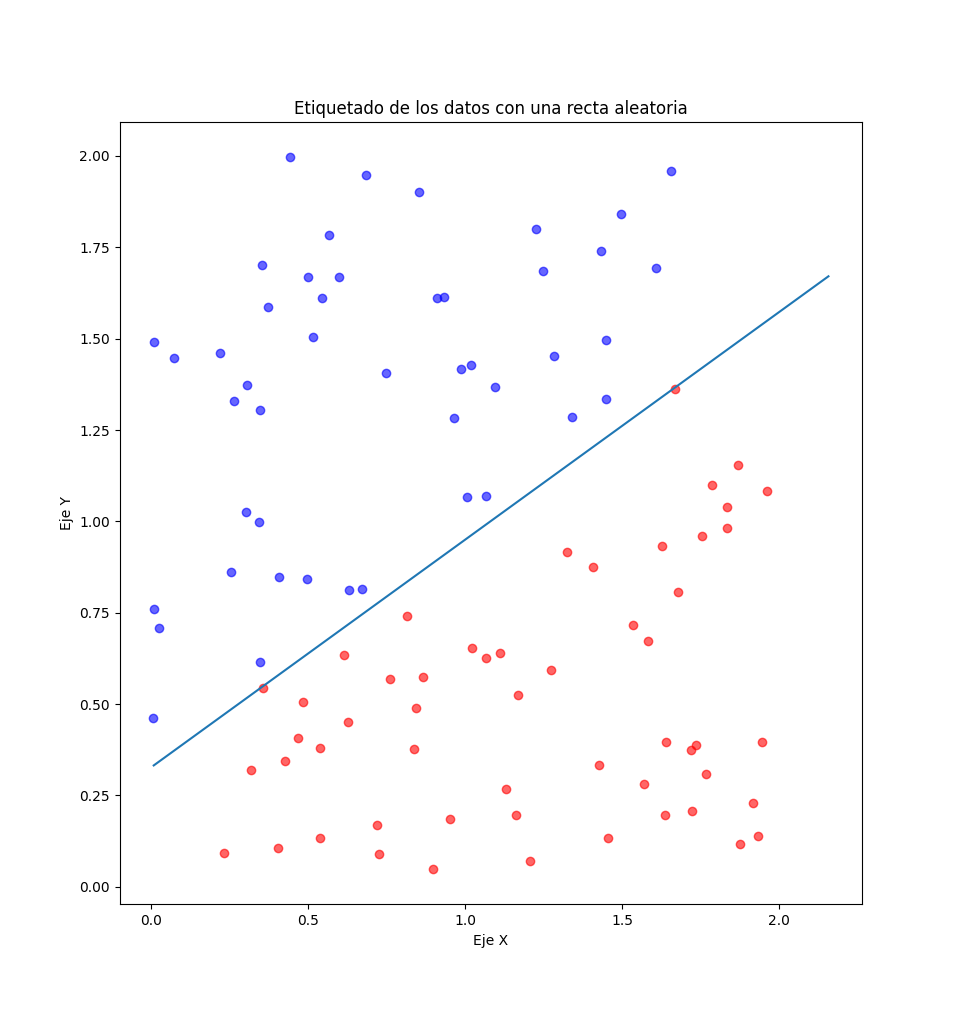
\includegraphics[scale=0.35]{frontera_resultado_lgr}
    \caption{Frontera solución junto al etiquetado original}
\end{figure}

Algunos puntos están más cercanos a la frontera que con la recta de etiquetado original. Con esto, podemos preveer que los puntos mal clasificados por el modelo estarán en esa zona fronteriza.

\subsubsection{Un ejemplo concreto de $E_{test}$}

Antes de lanzar los 100 experimentos, generamos un \emph{dataset} de test y mostramos cómo lo estamos haciendo fuera de la muestra. El tamaño de este \emph{test\_dataset} será de $10^4$ puntos. Este tamaño será también el usado en las 100 iteraciones del experimento.

Por pantalla mostramos que estamos fallando el $3.08\%$ de los datos del test. Es un valor razonable fuera de la muestra, por lo que podemos suponer que estamos generalizando bastante bien. Mostramos los puntos que han sido mal clasificados:

\begin{figure}[H]
    \centering
    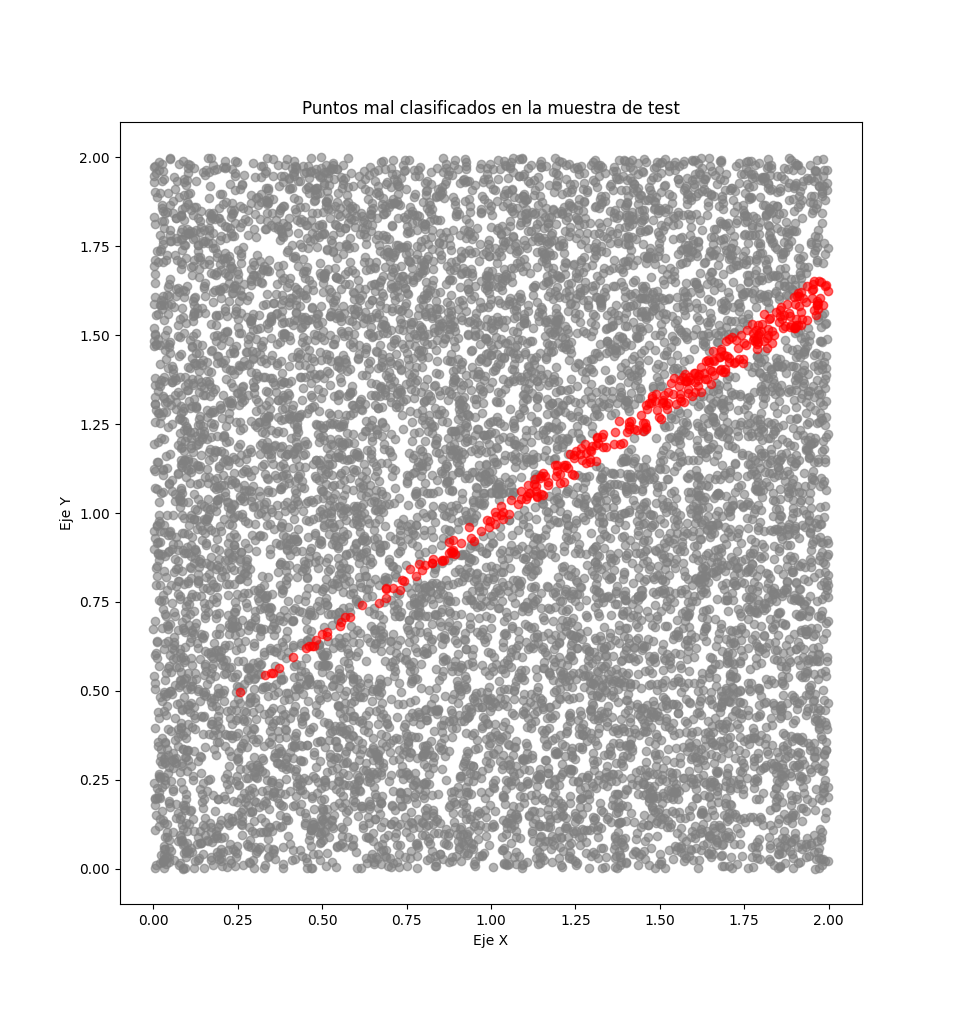
\includegraphics[scale=0.35]{lgr_puntos_mal_clasificados_test}
    \caption{Puntos mal clasificados en el conjunto de test}
\end{figure}

Y como ya habíamos comentado, los puntos mal clasificados se encuentran en la región fronteriza

\subsubsection{Experimento}

Lanzamos 100 veces el experimento y mostramos los resultados. En cada iteración del experimento, generamos una nueva muestra de datos (como en \ref{section:conjunto_datos_lgr}). Con una recta aleatoria, etiquetamos los datos. Lanzamos \emph{LGR-SGD} para este etiquetado. Generamos del mismo modo un \emph{test\_dataset} de $10^4$ puntos, etiquetados con la recta aleatoria. Y con esto, evaluamos el valor de $E_{test}$.

Este proceso es algo lento porque ya hemos visto que se necesitan muchas iteraciones de \emph{SGD} con \lstinline{batch_size = 1}.

El resultado que mostramos por pantalla es:

\begin{lstlisting}[caption={Resultado de las 100 iteraciones del experimento}, captionpos=b]
--> Media de iteraciones sobre minibatches consumidas: 40640.0
--> Media de iteraciones sobre epochs consumidas: 406.4
--> Media del porcentaje de puntos mal clasificados fuera de
    la muestra: 2.777%
--> Desviacion tipica del error fuera de la muestra: 0.01779
\end{lstlisting}

Estos resultados reafirman lo que hemos ido comentando. Notar que no estamos mostrando el error dentro de la muestra, pues al generar \emph{datasets} linealmente separables, potencialmente estamos alcanzando un $E_{in} = 0.0\%$. Este $E_{in} = 0.0\%$ debería hacernos pensar si estamos cometiendo \emph{overfitting} sobre la muestra de entrenamiento. Sin embargo la media de error fuera de la muestra es de $2.777\%$, por lo que estamos obteniendo una buena generalización.

Por otro lado, la desviación típica del error fuera de la muestra muestra una gran estabilidad de la capacidad de generalización fuera de la muestra, pues es un valor para la desviación muy bajo.

Es notable la gran cantidad de épocas que necesita \emph{SGD} para converger. Sin embargo, los buenos resultados justifican estos tiempos de entrenamiento.







\pagebreak


% Bibliografia
\bibliography{References}
\bibliographystyle{ieeetr}

\end{document}
